\documentclass[aspectratio=169,hyperref={pdfpagelabels=false,pageanchor=false,bookmarks=false}]{beamer}

% Beamer theme
\usefonttheme{professionalfonts}
\setbeamertemplate{navigation symbols}{}

% Math support
\usepackage{mathtools}

% Fonts
\usepackage[no-math]{fontspec}
\usepackage{microtype}
\defaultfontfeatures{Ligatures=TeX}
% Open source alternative to Gill Sans in UU's official layout
\usepackage[sfdefault]{gillius2}
\setmonofont{JuliaMono}[
Contextuals=Alternate,
Scale=MatchLowercase,
Extension=.ttf,
UprightFont=*-Regular,
BoldFont=*-Bold,
ItalicFont=*-RegularItalic,
BoldItalicFont=*-BoldItalic,
]
\usepackage{arevmath}
\usepackage{emoji}
\setemojifont{Noto Color Emoji}
\setbeamerfont{footnote}{size=\tiny}

% Languages
\usepackage{polyglossia}
\setdefaultlanguage{english}

% Graphics
\usepackage{graphicx}

% Tables
\usepackage{array}
\newcolumntype{P}[1]{>{\centering\arraybackslash}p{#1}}
\usepackage{booktabs}

% Colors
\def\UseCMYK{true}
\usepackage{UUcolorPantone}

% Boxes
\usepackage[export]{adjustbox}
\usepackage{tcolorbox}
\tcbset{shield externalize}
\tcbuselibrary{skins,raster}
\tcbset{coltitle=black,fonttitle=\bfseries\large\scshape}
\newenvironment{uuredbox}[1][]%
{\begin{tcolorbox}[colback=uured!15,colframe=uured,#1]}%
  {\end{tcolorbox}}
\newenvironment{uugreenbox}[1][]%
{\begin{tcolorbox}[colframe=gronskastark,#1]}%
  {\end{tcolorbox}}
\newenvironment{uuyellowbox}[1][]%
{\begin{tcolorbox}[colback=blondsvag,colframe=blondstark,#1]}%
  {\end{tcolorbox}}
\newenvironment{uubluebox}[1][]%
{\begin{tcolorbox}[colback=gryningmellan,colframe=gryningstark,#1]}%
  {\end{tcolorbox}}
\newenvironment{uugraybox}[1][]%
{\begin{tcolorbox}[colback=uulightgrey,colframe=black,#1]}%
  {\end{tcolorbox}}

% Tikz settings
\usetikzlibrary{graphs,graphs.standard,graphdrawing,patterns,positioning,calc,overlay-beamer-styles}
\usegdlibrary{force}
\usetikzlibrary{arrows,shapes,fadings}
\tikzset{
  block/.style={
    draw,
    rectangle,
    minimum height=1cm,
    minimum width=3cm, align=center
  },
  line/.style={->,>=latex'}
}

% Load PGFPlots and enable externalization
\usepackage{pgfplots}
\pgfplotsset{compat=1.18}
\usepgfplotslibrary{groupplots,fillbetween,units}
% Tufte style
\makeatletter
\def\pgfplotsdataxmin{\pgfplots@data@xmin}
\def\pgfplotsdataxmax{\pgfplots@data@xmax}
\def\pgfplotsdataymin{\pgfplots@data@ymin}
\def\pgfplotsdataymax{\pgfplots@data@ymax}
\makeatother
\pgfplotsset{
  range frame/.style={
    every axis legend/.append style={draw=none, fill=none, legend cell align=left},
    every axis/.append style={thick},
    tick style={thick,black},
    tick align=outside,
    scaled ticks=false,
    enlargelimits=false,
    axis lines*=left,
    line cap=round,
    clip=false,
    axis line shift=5pt,
    colorbar style={
      tick align=outside,
      ytick pos=right,
    },
  }
}
% Colorbrewer
\usepgfplotslibrary{colorbrewer}
\pgfplotsset{
  % Initialize Dark2-8:
  cycle list/Dark2-8,
  % Combine it with ’mark list*’:
  cycle multiindex* list={
    mark list*\nextlist
    Dark2-8\nextlist
    linestyles\nextlist
  },
}
\usepgfplotslibrary{external}
\tikzset{external/only named=true}
\directlua{os.execute("mkdir -p tikzcache")}
\tikzexternalize[prefix=tikzcache/]
% Adjust font sizes
\pgfplotsset{
  every axis legend/.append style={font=\footnotesize},
  every tick label/.append style={font=\footnotesize},
  every axis label/.append style={font=\footnotesize},
  every axis title/.append style={font=\small},
}

% Fix externalization of overlays (one image per overlay)
\makeatletter
\newcommand*{\overlaynumber}{\number\beamer@slideinframe}
\tikzset{
  beamer externalizing/.style={%
    execute at end picture={%
      \tikzifexternalizing{%
        \ifbeamer@anotherslide
        \pgfexternalstorecommand{\string\global\string\beamer@anotherslidetrue}%
        \fi
      }{}%
    }%
  },
  external/optimize=false
}
\let\orig@tikzsetnextfilename=\tikzsetnextfilename
\renewcommand\tikzsetnextfilename[1]{\orig@tikzsetnextfilename{#1-\overlaynumber}}
\makeatother
\tikzset{every picture/.style={beamer externalizing}}

% Highlighting
\newcommand\hl[1]{\begingroup\bfseries\boldmath\color{red}#1\endgroup}

% References
\usepackage[style=authortitle-icomp,doi=false,url=false,isbn=false,uniquename=init,giveninits=true]{biblatex}
\addbibresource{references.bib}
\DeclareCiteCommand{\citeauthorfirstlast}
{\boolfalse{citetracker}%
  \boolfalse{pagetracker}%
  \DeclareNameAlias{labelname}{given-family}%
  \usebibmacro{prenote}}
{\ifciteindex
  {\indexnames{labelname}}
  {}%
  \printnames{labelname}}
{\multicitedelim}
{\usebibmacro{postnote}}

% Footnotes
\usepackage{hanging}
\setbeamertemplate{footnote}{%
  \usebeamercolor{footnote}%
  \hangpara{2em}{1}\makebox[2em][r]{\insertfootnotemark}\insertfootnotetext\par%
}
\usepackage{fontawesome}
\newcommand{\reffootnote}[1]{%
  \let\oldthefootnote=\thefootnote%
  \addtocounter{footnote}{-1}%
  \renewcommand{\thefootnote}{}%
  \footnote{\hspace{-2em}\hbox to 2em{\hfil\faBook\hspace{0.2em}}\fullcite{#1}}%
  \let\thefootnote=\oldthefootnote%
}

\newenvironment{refitemize}%
{%
  \noindent\rule{\textwidth}{0.4pt}\par%
  \vspace*{-\parskip}%
  \setbeamertemplate{itemize item}{\leavevmode\tiny\includegraphics[raise=-2pt,width=5pt]{beamericonarticle}}%
  \setbeamerfont{itemize/enumerate body}{size=\tiny}%
  \setlength\topsep{0pt}%NEW
  \setlength\partopsep{0pt}%NEW
  \setlength\itemsep{0pt}%NEW
  \settowidth{\leftmargini}{\usebeamertemplate{itemize item}}%
  \addtolength{\leftmargini}{\labelsep}%
  \begin{itemize}%
          }{%
  \end{itemize}%
  \par\ignorespacesafterend%
}
\newcommand\refitem[1]{\item \fullcite{#1}}

% Code
\tcbuselibrary{minted,breakable}
\newtcblisting{juliaconsnippet}[1][]{%
  blank,
  listing engine=minted,
  minted language={jlcon},
  minted options={autogobble,breaklines,mathescape,fontsize=\footnotesize},
  listing only,
  breakable,
  sharp corners,
  colback=black!5,
  boxrule=1pt,
  leftrule=0pt,
  rightrule=0pt,
  left=0pt,
  top=0pt,
  bottom=0pt,
  right=0pt,
  #1
}

% Quotes (should be loaded after minted)
\usepackage{csquotes}

% Draw scratch counts
\usepackage{luamplib}
\newcommand{\scratchcount}[1]{%
  \begin{mplibcode}
    beginfig(0);
    n:= #1;
    height := 3/5\mpdim{\normalbaselineskip} ;
    span := 1/3 * height ;
    drift := 1/10 * height ;
    pickup pencircle scaled (1/12 * height) ;
    def d = (uniformdeviate drift) enddef ;
    for i := 1 upto n :
    draw
    if (i mod 5)=0 : ((-d-4.5span,d)--(+d-0.5span,height-d))
    else : ((-d,+d)--(+d,height-d)) fi
    shifted (span*i,d-drift) ;
    endfor;
    endfig;
  \end{mplibcode}}


\DeclareMathOperator{\law}{law}
\DeclareMathOperator{\ECE}{ECE}
\DeclareMathOperator{\Dir}{Dir}
\DeclareMathOperator{\Categorical}{Cat}

% there is an issue with \widehat and \DeclareMathOperator
\makeatletter
\newcommand*{\biasedestimator}{\widehat{\operator@font SKCE}_{\operator@font b}}
\newcommand*{\unbiasedestimator}{\widehat{\operator@font SKCE}_{\operator@font uq}}
\newcommand*{\linearestimator}{\widehat{\operator@font SKCE}_{\operator@font ul}}
\makeatother

\setbeamersize{description width=2cm}
% Adapted from default in beamer/base/themes/inner/beamerinnerthemedefault.sty
% without section number
\setbeamertemplate{section page}
{
  \begingroup
  \centering
  \begin{beamercolorbox}[sep=12pt,center]{section title}
    \usebeamerfont{section title}\insertsection\par
  \end{beamercolorbox}
  \endgroup
}

% Download picture from the web, if necessary
\IfFileExists{figures/penguins.png}{}{%
  \write18{curl -o ./figures/penguins.png --create-dirs https://raw.githubusercontent.com/allisonhorst/palmerpenguins/69530276d74b99df81cc385f4e95c644da69ebfa/man/figures/lter_penguins.png}
}

\title{Calibration of probabilistic predictive models}
\subtitle{Machine Learning Journal Club, Gatsby Unit}
\date{28 March 2022}
\author{David Widmann}
\titlegraphic{%
	\begin{tikzpicture}[overlay,remember picture]
		\node[xshift=-1cm,yshift=-1cm,inner sep=0pt,outer sep=0pt] at (current page.north east) {
\includegraphics[height=1.25cm]{figures/UU.pdf}};
	\end{tikzpicture}%
}
\institute{%
  \href{https://www.it.uu.se/}{Department of Information Technology, Uppsala University, Sweden}\\%
  \href{https://www.math.uu.se/research/cim/}{Centre for Interdisciplinary Mathematics, Uppsala University, Sweden}%
}

% Useful for adding email address to title page:
% https://tex.stackexchange.com/a/376474
\def\vfilll{\vskip 0pt plus 1filll minus 0pt }

\begin{document}
\NoHyper

\begin{frame}
  \vfilll
  \titlepage
  \vfilll
  {%
    \usebeamerfont{institute}%
    Contact: \href{mailto:david.widmann@it.uu.se}{\texttt{david.widmann@it.uu.se}}%
  }
\end{frame}

% Introduce myself
\begin{frame}{About me}
  % Summary
  \only<1>{%
    \begin{columns}
      \begin{column}{0.75\textwidth}
        \begin{block}{TL;DR \emoji{book}}
          \begin{itemize}
            \item 31 year old PhD student at Uppsala University
            \item On parental leave since September 2021
            \item Research on uncertainty quantification of probabilistic models
            \item Active member in the Julia community
          \end{itemize}
        \end{block}
      \end{column}
      \begin{column}{0.25\textwidth}
        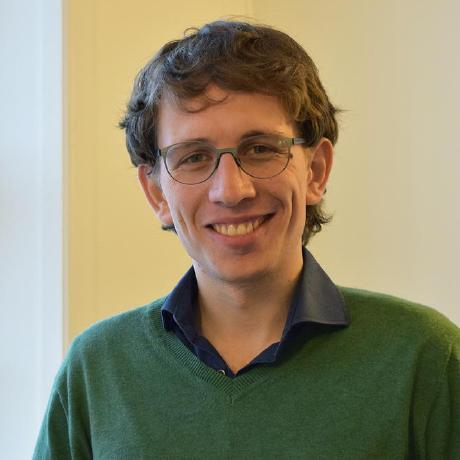
\includegraphics[width=\linewidth]{figures/profile.jpg}
      \end{column}
    \end{columns}}
  % Education
  \only<2-3>{%
    \begin{block}{Education \emoji{graduation-cap}}
      \begin{description}
        \item[2017---now:] PhD student (Uppsala University)
        \item[2016---2017:] MSc Mathematics (TU Munich)
        \item[2013---2016:] BSc Mathematics (TU Munich)
        \item[2007---2013:] Human medicine (LMU and TU Munich)
      \end{description}
    \end{block}%
    % Research interests
    \onslide<3>{%
      \begin{block}{Research interests \emoji{microscope}}
        \begin{itemize}
          \item Research topic: "Uncertainty-aware deep learning"
          \item Statistics, probability theory, scientific machine learning, and computer science
          \item Julia programming, e.g., \href{https://sciml.ai}{SciML} and \href{https://turing.ml}{Turing}
        \end{itemize}
      \end{block}}}
\end{frame}

\begin{frame}{Papers}
  \begin{itemize}
    \item \fullcite{Vaicenavicius2019}
          \begin{itemize}
            \item Focus on multi-class classification, calibration lenses, calibration estimation and tests with ECE
          \end{itemize}
          \pause
    \item \fullcite{Widmann2019}
          \begin{itemize}
            \item Calibration errors and tests for multi-class classification based on matrix-valued kernels
          \end{itemize}
          \pause
    \item \fullcite{Widmann2021}
          \begin{itemize}
            \item Calibration errors and tests for probabilistic predictive models based on scalar-valued kernels
          \end{itemize}
  \end{itemize}
\end{frame}

\section{Calibration: Motivation and definition}
\frame{\sectionpage}

\begin{frame}{Example: Weather forecasts}
  \begin{columns}[t]
    \begin{column}{0.5\textwidth}
      \begin{figure}
        \centering
        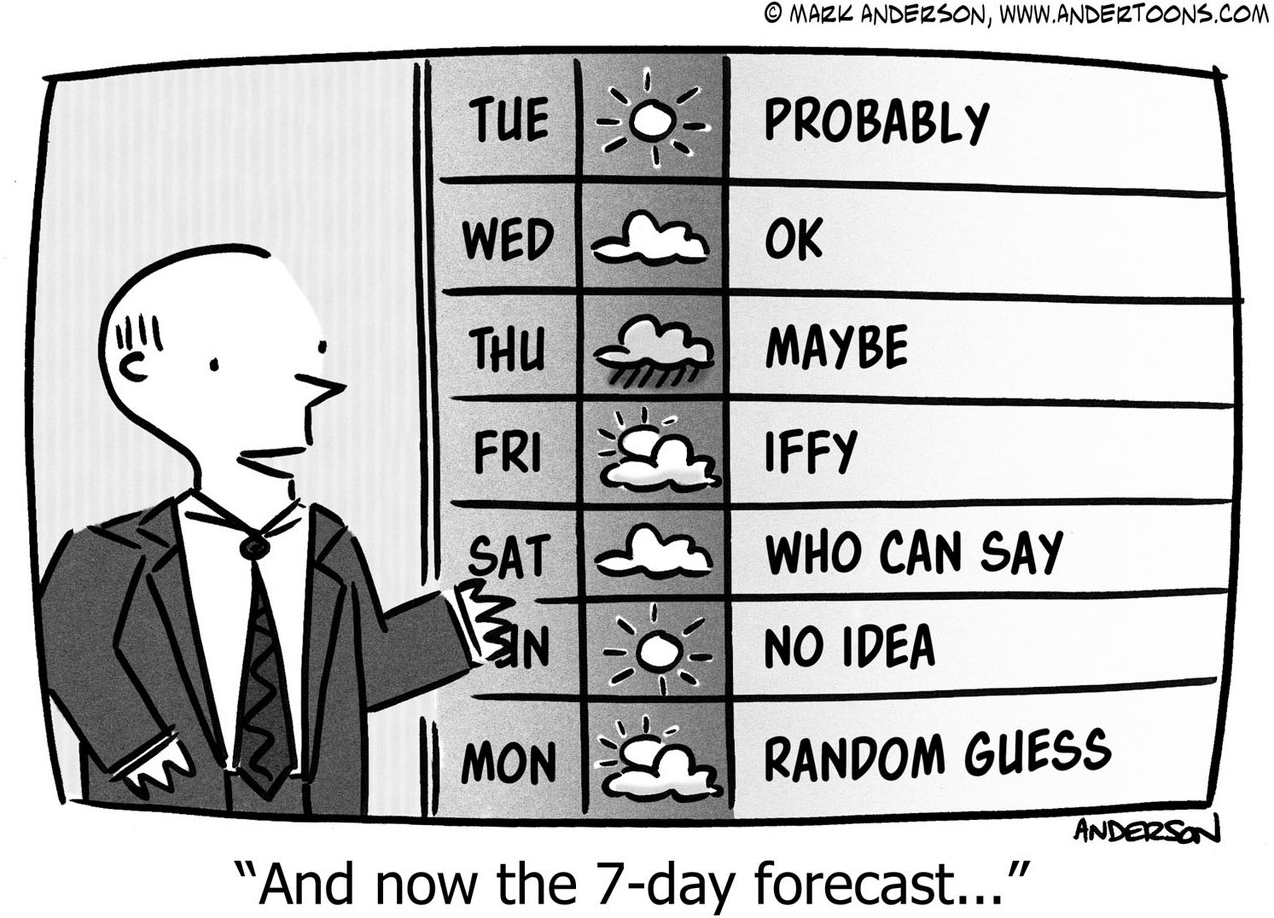
\includegraphics[width=\textwidth]{figures/forecaster.png}
      \end{figure}
    \end{column}%
    \pause%
    \begin{column}{0.5\textwidth}
      \enquote{%
        Those forecasts which were marked \enquote{doubtful} were the
        \emph{best I could frame} under the circumstances. \textelp{} If I
        make no distinction between these and others, I degrade the whole.}
      \vskip5mm
      \hspace*\fill{\small ---\citeauthorfirstlast{Cooke1906B}}%
    \end{column}%
  \end{columns}
  \reffootnote{Cooke1906B}
\end{frame}

\begin{frame}{Motivation: Classification example}
  \only<1>{%
    \begin{figure}
      \tikzsetnextfilename{penguins}
      \begin{tikzpicture}
        \begin{axis}[
          range frame,
          legend pos=outer north east,
          xlabel=bill length,
          ylabel=flipper length,
          use units,
          x unit=mm,
          y unit=mm,
          height=0.7\textheight,
          scatter/classes={
            Adelie={mark=square*, Dark2-B},
            Chinstrap={mark=triangle*, Dark2-C},
            Gentoo={mark=*, Dark2-A}
          },
          ]

          \addplot+ [
          scatter,
          fill opacity=0,
          only marks,
          scatter src=explicit symbolic,
          prefix = pgfshell_,
          id = penguins,
          ] table [
          x=bill_length_mm, y=flipper_length_mm, meta=species, header=true
          ] shell {
            curl -s https://raw.githubusercontent.com/allisonhorst/palmerpenguins/69530276d74b99df81cc385f4e95c644da69ebfa/inst/extdata/penguins.csv | awk '
            BEGIN { FS = ","; }
            NR==1 {
              for (i=1; i<=NF; i++) {
                f[$i] = i;
              };
            }
            {
              bill = $(f["bill_length_mm"]);
              flipper = $(f["flipper_length_mm"]);
              species = $(f["species"]);
              if (bill != "NA" && flipper != "NA" && species != "NA") {
                print bill, flipper, species;
              };
            }
            '
          };
          \legend{Adélie, Chinstrap, Gentoo};
        \end{axis}
      \end{tikzpicture}
    \end{figure}
    \reffootnote{Gorman2014}%
  }%
  \only<2-3>{%
    \begin{figure}
      \centering
      \begin{tikzpicture}
        \node (model) at (0, 0)
        {\includegraphics[height=0.15\textheight]{figures/model.pdf}};
        \node[above=0.8cm of model, font=\large\bfseries] (label) {Model $P$};
        \node[left=1cm of model] (input) {\includegraphics[width=0.2\textwidth]{figures/measure.pdf}};
        \node[anchor=base, font=\large\bfseries] at (input|-label.base) {Input $X$};
        \draw[line] (input) -- (model);
        \node[right=1cm of model] (prediction)
        {
          \includegraphics[width=0.3\textwidth]{figures/penguins.png}
        };
        \node [font=\large\bfseries, align=center] at (label-|prediction) {Prediction $P_X$\\(distribution of target $Y$)};
        \node [below=0mm of prediction, font=\tiny, anchor=west] {Artwork by \texttt{@allison\_horst}};
        \draw [line] (model) -- (prediction);
      \end{tikzpicture}
    \end{figure}
    \onslide<3->{
      \begin{block}{Example: Prediction $P_{X}$}
        \begin{center}
          \begin{tabular}{@{}ccc@{}}
            \textcolor{Dark2-B}{\texttt{Adélie}} & \textcolor{Dark2-C}{\texttt{Chinstrap}} & \textcolor{Dark2-A}{\texttt{Gentoo}} \\ \midrule
            80\% & 10\% & 10\% \\
          \end{tabular}
        \end{center}
      \end{block}
    }%
  }
\end{frame}

\begin{frame}{Calibration: Intuition}
  \begin{figure}
    \begin{tikzpicture}
      \node (model) at (0, 0)
      {\includegraphics[height=0.15\textheight]{figures/model.pdf}};
      \node[above=0.5cm of model, font=\large\bfseries] (label) {Model $P$};
      \onslide<2->{%
        \node [left=1cm of model, name=feature] {%
          Input \alt<2-4>{$x_1$}{\alt<5-7>{$x_2$}{\alt<8-10>{$x_3$}{$x_i$}}}};
        \draw [line] (feature) -- (model);
      }
      \visible<3,4,6,7,9-11>{%
        \node[right=1cm of model, align=left, minimum height=0.15\textwidth] (prediction)
        {%
          \begin{tabular}{@{}ccc@{}}
            \textcolor{Dark2-B}{\texttt{Adelie}} & \textcolor{Dark2-A}{\texttt{Chinstrap}} & \textcolor{Dark2-C}{\texttt{Gentoo}} \\ \midrule
            80\% & 10\% & 10\% \\
          \end{tabular}};
        \draw [line] (model) -- (prediction);
        \node [font=\large\bfseries, anchor=base, align=center] at (label.base-|prediction) {Prediction \alt<3-4>{$P_{x_{1}}$}{\alt<6,7>{$P_{x_{2}}$}{\alt<9,10>{$P_{x_{3}}$}{$P_{x_{i}}$}}}};
      }
    \end{tikzpicture}
  \end{figure}

  \onslide<4->{%
    \begin{block}{Empirical frequency}
      \begin{center}
        \directlua{math.randomseed(101)}
        \begin{tabular}{@{}ccc@{}}
          \textcolor{Dark2-B}{\texttt{Adelie}} & \textcolor{Dark2-A}{\texttt{Chinstrap}} & \textcolor{Dark2-C}{\texttt{Gentoo}} \\ \midrule
          \alt<4-9>{\scratchcount{1}}{\alt<10>{\scratchcount{2}}{\scratchcount{8} \ldots}} & \alt<-6>{}{\alt<7-10>{\scratchcount{1}}{\scratchcount{2} \ldots}} & \alt<4-10>{}{\scratchcount{1} \ldots} \\
        \end{tabular}
      \end{center}
    \end{block}
  }%
\end{frame}

\begin{frame}{Calibration}
  \begin{tcbraster}[raster columns=2,raster equal height=rows]
    \onslide<2->{%
      \begin{tcolorbox}[blankest, raster multicolumn=2, halign=flush center, bottom=0.5cm]
        \large\hl{Predictions consistent with empirically observed frequencies?}
      \end{tcolorbox}}%
    \begin{tcolorbox}[blanker, title={Prediction $P_{X}$}, center title, valign=center, remember as=B]
      \begin{center}
        \begin{tabular}{@{}ccc@{}}
          \textcolor{Dark2-B}{\texttt{Adélie}} & \textcolor{Dark2-C}{\texttt{Chinstrap}} & \textcolor{Dark2-A}{\texttt{Gentoo}} \\ \midrule
          80\% & 10\% & 10\% \\
        \end{tabular}
      \end{center}
    \end{tcolorbox}
    \begin{tcolorbox}[blanker, title={Empirical frequency $\law(Y \,|\, P_X)$}, center title, valign=center, remember as=A]
      \directlua{math.randomseed(101)}
      \begin{center}
        \begin{tabular}{@{}ccc@{}}
          \textcolor{Dark2-B}{\texttt{Adélie}} & \textcolor{Dark2-C}{\texttt{Chinstrap}} & \textcolor{Dark2-A}{\texttt{Gentoo}} \\ \midrule
          \scratchcount{8} \ldots & \scratchcount{2} \ldots & \scratchcount{1} \ldots \\
        \end{tabular}
      \end{center}
    \end{tcolorbox}
  \end{tcbraster}
  \onslide<2->{%
    \begin{tikzpicture}[remember picture, overlay]
      \path (A) -- node [font=\bfseries\boldmath\Huge, color=red, align=center, midway] {$\stackrel{\text{?}}{=}$} (B);
    \end{tikzpicture}}
  \onslide<3->{%
    \begin{definition}
      A probabilistic predictive model $P$ is calibrated if
      \begin{equation*}
        \law(Y \,|\, P_X) = P_X \qquad \text{almost surely}.
      \end{equation*}
    \end{definition}
  }
  \onslide<4->{%
    \begin{tcolorbox}[blankest, halign=flush center]
      Notion captures also weaker confidence calibration
    \end{tcolorbox}}
  \reffootnote{Widmann2019}
  \reffootnote{Widmann2021}
\end{frame}

\begin{frame}{Binary classification: Reliability diagram}
  \only<1-4>{%
    \begin{figure}
      \tikzsetnextfilename{reliability_diagram-\overlaynumber}
      \begin{tikzpicture}
        \begin{axis}[
          range frame,
          axis equal image,
          height = 0.7\textheight,
          xlabel = prediction,
          ylabel = empirical frequency,
          xmin = 0, xmax = 1,
          ymin = 0, ymax = 1,
          domain = 0:1,
          ]
          \addplot+ [black, dashed, mark=none, samples=2] {x};
          \addplot+ [Dark2-A, solid, mark=none, visible on=<2->, samples=100] {x*(1+(x-1.5)*(x-0.6))};
          [sloped]
          node [pos=0.3, above, visible on=<3->] {underconfident};
          node [pos=0.85, below, visible on=<4->] {overconfident};
        \end{axis}
      \end{tikzpicture}
    \end{figure}}%
  \only<5>{%
    \begin{figure}
      \tikzsetnextfilename{reliability_diagram_variant}
      \begin{tikzpicture}
        \begin{axis}[
          range frame,
          height = 0.7\textheight,
          xlabel = prediction,
          ylabel = deviation,
          xmin = 0, xmax = 1,
          domain = 0:1,
          ]
          \addplot+ [black, dashed, mark=none, samples=2] {0};
          \addplot+ [Dark2-A, solid, mark=none, samples=100] {x*(x-1.5)*(x-0.6)};
          node [pos=0.3, above] {underconfident};
          node [pos=0.8, sloped, below] {overconfident};
        \end{axis}
      \end{tikzpicture}
    \end{figure}}%
  \reffootnote{Vaicenavicius2019}
\end{frame}

\begin{frame}{Multi-class classification: All scores matter!}
  \begin{tcbraster}[raster columns=1]
    \begin{tcolorbox}[blankest]
      \begin{center}
        \begin{tikzpicture}
          \node[minimum height=0.11\textwidth, inner sep=2mm] (image) at (0, 0)
          {\begin{tabular}{@{}ccc@{}}
             \includegraphics[height=3mm]{figures/car0.pdf} & \includegraphics[height=3mm]{figures/car1.pdf} & \includegraphics[height=3mm]{figures/car2.pdf} \\
             \includegraphics[height=3mm]{figures/car3.pdf} & \includegraphics[height=3mm]{figures/car4.pdf} & $\cdots$ \\
           \end{tabular}};

         \onslide<2->{%
           \node[right=1cm of image, inner sep=2mm] (model)
           {\includegraphics[height=\dimexpr0.11\textwidth-4mm\relax]{figures/model.pdf}};
           \draw [->] (image) -- (model);
         }%

         \onslide<3->{%
           \node[right=1cm of model, minimum height=0.11\textwidth, align=center] (prediction)
           {\begin{tabular}{@{}ccc@{}}
              \texttt{object} & \texttt{human} & \texttt{animal} \\ \midrule
              80\% & 0\% & 20\% \\
            \end{tabular}};
          \draw [->] (model) -- (prediction);
        }%
      \end{tikzpicture}
    \end{center}
  \end{tcolorbox}
  \onslide<4->{%
    \begin{uubluebox}
      \begin{center}
        Common calibration evaluation techniques consider only the
        most-confident score
      \end{center}
    \end{uubluebox}
  }%
  \onslide<5-> & 0\% & 20\% \\
          \hl{80\%} & 20\% & 0\% \\ \bottomrule
        \end{tabular}
      \end{center}
    \end{uuredbox}
  }%
\end{tcbraster}
\reffootnote{Vaicenavicius2019}
\end{frame}

\begin{frame}{Weaker notions of calibration and calibration lenses}
  \begin{block}{Weaker notions}
    Weaker notions of calibration such as confidence calibration or calibration of marginal classifiers can be analyzed by considering calibration of induced predictive models.
  \end{block}
  \pause
  \begin{definition}[Calibration lenses]
    Let $\psi$ be a measureable function that defines targets $Z := \psi(Y, P_{X})$.
    Then $\psi$ induces a predictive model $Q$ for targets $Z$ with predictions
    \begin{equation*}
      Q_{X} := \law\big(\psi(\tilde{Y}, P_{X})\big)
    \end{equation*}
    where $\tilde{Y} \sim P_{X}$.
    Function $\psi$ is called a \emph{calibration lens}.
  \end{definition}
  \reffootnote{Vaicenavicius2019}
\end{frame}

\begin{frame}{Beyond classification}
  \begin{definition}[reminder]
    A probabilistic predictive model $P$ is calibrated if
    \begin{equation*}
      \law(Y \,|\, P_X) = P_X \qquad \text{almost surely}.
    \end{equation*}
  \end{definition}

  \pause

  \begin{block}{Examples of other target spaces}
    \begin{tcbraster}[blankest, raster columns=4,raster equal height=rows, halign=flush center]
      \begin{tcolorbox}
        $\mathbb{N}_0$\\[\baselineskip]
        \begin{tikzpicture}[scale=0.5]
          \begin{axis}[
            range frame,
            xlabel=$X$,
            ylabel=$Y$,
            height=0.6\textheight,
            domain=-20:60,
            bar width=2,
            ]
            \pgfmathsetseed{1234}
            \addplot+ [ybar, no marks, samples=20] ({x + 0.1*rand}, {round(50*rnd)});
          \end{axis}
        \end{tikzpicture}
      \end{tcolorbox}
      \begin{tcolorbox}
        $\mathbb{R}^d$\\[\baselineskip]
        \begin{tikzpicture}[scale=0.5]
          \begin{axis}[
            range frame,
            xlabel=$X$,
            ylabel=$Y$,
            height=0.6\textheight,
            domain=-20:60,
            ]
            \addplot+ [no marks, samples=2] {5 + 0.1*x};

            \pgfmathsetseed{1234}
            \addplot+ [only marks, mark=*, mark size=0.75, samples=70] ({x + 0.1*rand}, {5 + 0.1*x + 3*rand});
          \end{axis}
        \end{tikzpicture}
      \end{tcolorbox}
      \begin{tcolorbox}
        graphs\\[\baselineskip]
        \begin{tikzpicture}[scale=0.5]
          \pgfmathsetseed{1234}
          \graph [spring layout, nodes={draw, scale=0.5, circle, fill=Dark2-B, as=}, n=25, p=0.3] {
            subgraph I_n;
            subgraph G_np
          };
        \end{tikzpicture}
      \end{tcolorbox}
      \begin{tcolorbox}
        protein structure\\[\baselineskip]
        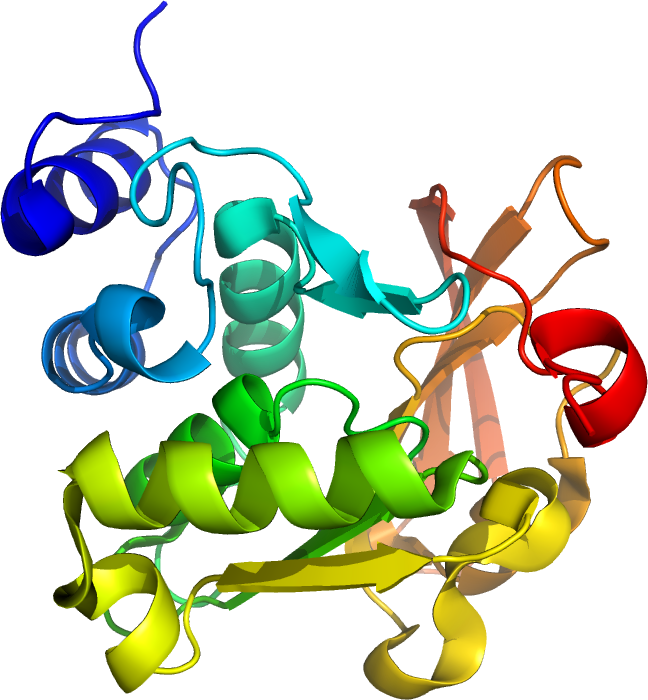
\includegraphics[height=0.25\textheight]{figures/protein.png}%
      \end{tcolorbox}
    \end{tcbraster}
  \end{block}
  \reffootnote{Widmann2021}
\end{frame}

\section{Calibration errors}
\frame{\sectionpage}

\begin{frame}{Expected calibration error (ECE)}
  \begin{definition}
    The expected calibration error ($\operatorname{ECE}$) with respect to
    distance measure $d$ is defined as
    \begin{equation*}
      \operatorname{ECE}_d := \mathbb{E}_{P_X} d\big(P_X, \law(Y\,|\, P_X)\big).
    \end{equation*}
  \end{definition}
  \pause
  \begin{block}{Choice of distance measure $d$}
    \begin{itemize}[<+->]
      \item For classification typically (semi-)metrics on the probability simplex
            (e.g., cityblock, Euclidean, or squared Euclidean distance)
      \item For general probabilistic predictive models \hl{statistical divergences}
    \end{itemize}
  \end{block}
\end{frame}

\begin{frame}{Statistical divergences}
  \begin{definition}
    Let $\mathcal{P}$ be a space of probability distributions.
    A function $d \colon \mathcal{P} \times \mathcal{P} \to \mathbb{R}$ that satisfies
    \begin{itemize}
      \item $d(P, Q) \geq 0$ for all $P, Q \in \mathcal{P}$,
      \item $d(P, Q) = 0$ if and only if $P = Q$,
    \end{itemize}
    is a statistical divergence.
  \end{definition}
  \pause
  \begin{block}{Note}
    \begin{itemize}
      \item $d$ does not need to be symmetric
      \item $d$ does not need to satisfy the triangle inequality
    \end{itemize}
  \end{block}
  \pause
  \begin{block}{Examples}
    \begin{itemize}
      \item $f$-divergences, e.g., Kullback-Leibler divergence or total variation distance
      \item Wasserstein distance
    \end{itemize}
  \end{block}
\end{frame}

\begin{frame}{Scoring rules: Definition}
  \begin{definition}
    The expected score of a probabilistic predictive model $P$ is defined as
    \begin{equation*}
      \operatorname{\mathbb{E}}_{P_X, Y} s(P_X, Y)
    \end{equation*}
    where \hl{scoring rule $s(p, y)$} is the reward of prediction $p$ if the true outcome is $y$.
  \end{definition}
  \pause
  \begin{block}{Examples for classification}
    \begin{itemize}
      \item Brier score: $s(p, y) = - \int_{\Omega} \big((\delta_{y} - p)^2\big)(\mathrm{d}\omega)$
      \item Logarithmic score: $s(p, y) = \log p\big(\{y\}\big)$
    \end{itemize}
  \end{block}
\end{frame}

\begin{frame}{Scoring rules: Decomposition}
  For proper scoring rules
  \begin{equation*}
    \begin{split}
      \operatorname{\mathbb{E}}_{P_X, Y} s(P_X, Y) ={}& \alt<1>{\vphantom{\underbrace{\operatorname{\mathbb{E}}_{P_X} d(\law(Y), \law(Y \,|\, P_X))}_{\mathclap{\text{resolution}}}}\operatorname{\mathbb{E}}_{P_X} d(\law(Y), \law(Y \,|\, P_X))}{\underbrace{\operatorname{\mathbb{E}}_{P_X} d(\law(Y), \law(Y \,|\, P_X))}_{\mathclap{\text{resolution}}}} \\
      &{-} \alt<1-2>{\vphantom{\underbrace{\operatorname{\mathbb{E}}_{P_X} d(P_X, \law(Y \,|\, P_X))}_{\mathclap{\text{\hl{calibration}}}}}\operatorname{\mathbb{E}}_{P_X} d(P_X, \law(Y \,|\, P_X))}{\underbrace{\operatorname{\mathbb{E}}_{P_X} d(P_X, \law(Y \,|\, P_X))}_{\mathclap{\text{\hl{calibration}}}}} {-} \alt<1-3>{\vphantom{\underbrace{S(\law(Y), \law(Y))}_{\mathclap{\text{uncertainty of }Y}}}S(\law(Y), \law(Y))}{\underbrace{S(\law(Y), \law(Y))}_{\mathclap{\text{uncertainty of }Y}}}
    \end{split}
  \end{equation*}
  \begin{columns}
    \begin{column}{0.5\textwidth}
      \begin{block}{Expected score of $P$ under $Q$}
        \vspace*{-\baselineskip}
        \begin{equation*}
          S(P, Q) := \int_{\Omega} s(P, \omega) \,Q(\mathrm{d}\omega)
        \end{equation*}
      \end{block}
    \end{column}
    \begin{column}{0.5\textwidth}
      \begin{block}{Score divergence}
        \vspace*{-\baselineskip}
        \begin{equation*}
          \vphantom{S(P, Q) := \int_{\Omega} s(P, \omega) \,Q(\mathrm{d}\omega)}d(P, Q) = S(Q, Q) - S(P, Q)
        \end{equation*}
      \end{block}
    \end{column}
  \end{columns}%
  \onslide<5>{%
    \begin{center}
      \hl{Models can trade off calibration for resolution!}
    \end{center}}
  \reffootnote{Broecker2009}
\end{frame}

\begin{frame}{An alternative definition of calibration}
  \begin{theorem}
    A probabilistic predictive model $P$ is calibrated if
    \begin{equation*}
      (P_X, Y) \stackrel{d}{=} (P_X, Z_X),
    \end{equation*}
    where $Z_X \sim P_X$.
  \end{theorem}
  \onslide<2>{%
    \begin{uugreenbox}[halign=flush center]
      Calibration error as distance between $\law\big((P_X, Y)\big)$ and $\law\big((P_X, Z_X)\big)$
    \end{uugreenbox}}
  \reffootnote{Widmann2021}
\end{frame}

\begin{frame}{Calibration error: Integral probability metric}
  \begin{tcolorbox}[blankest]
    \vspace*{-\baselineskip}
    \begin{equation*}
      \operatorname{CE}_{\mathcal{F}} := \sup_{f \in \mathcal{F}} \Big| \operatorname{\mathbb{E}}_{P_X,Y} f(P_X,Y) - \operatorname{\mathbb{E}}_{P_X,Z_X} f(P_X,Z_X)\Big|
    \end{equation*}
  \end{tcolorbox}
  \onslide<2->{%
    \begin{block}{Examples}
      \begin{itemize}[<+->]
        \item 1-Wasserstein distance: $\mathcal{F} = \{f \colon \|f\|_{\operatorname{Lip}} \leq 1\}$
        \item Total variation distance: $\mathcal{F} = \{f \colon \|f\|_{\infty} \leq 1\}$
      \end{itemize}
    \end{block}%
  }
  \onslide<3->{%
    \begin{uugreenbox}[halign=flush center]
      Common choices of $\operatorname{ECE}_d$ in classification can be formulated in this way
    \end{uugreenbox}%
  }
  \reffootnote{Widmann2019}
  \reffootnote{Widmann2021}
\end{frame}

\begin{frame}{Kernel calibration error: Maximum mean discrepancy (MMD)}
  \begin{tcolorbox}[blankest]
    Choose $\mathcal{F} = \{f \in \mathcal{H}\colon \|f\|_{\mathcal{H}} \leq 1\}$ for some reproducing kernel Hilbert space $\mathcal{H}$
  \end{tcolorbox}
  \onslide<2->{%
    \begin{block}{Reproducing kernel Hilbert space (RKHS)}
      \begin{itemize}
        \item<2-> Hilbert space of functions that satisfy $f \text{ close to } g \Rightarrow f(x) \text{ close to } g(x)$
        \item<3-> Possesses a positive-definite function $k$ as reproducing kernel
      \end{itemize}
    \end{block}%
  }
  \onslide<4->{%
    \begin{definition}
      The kernel calibration error ($\operatorname{KCE}$) of a model $P$ with respect to kernel $k$ is defined as
      \begin{equation*}
        \operatorname{KCE}^2_k := \operatorname{CE}^2_{\mathcal{F}} =
        \int k\big((p, y), (\tilde{p}, \tilde{y})\big) \, \mu\big(\mathrm{d}(p, y)\big) \mu\big(\mathrm{d}(\tilde{p}, \tilde{y})\big),
      \end{equation*}
      where $\mu = \law\big((P_X, Y)\big) - \law\big((P_X, Z_X)\big)$.
    \end{definition}%
  }
  \reffootnote{Widmann2019}
  \reffootnote{Widmann2021}
\end{frame}

\begin{frame}{Choice of kernel}
  \begin{block}{Observations}
    \begin{itemize}[<+->]
      \item Kernel $k$ defined on the product space of predictions and targets
      \item In multi-class classification, $k$ can be identified with a matrix-valued kernel on the space of predictions
      \item For specific kernel choices, $Z_{X}$ can be integrated out analytically
      \item Otherwise numerical integration methods (e.g., Monte Carlo integration) can be used to integrate out $Z_{X}$
      \item Suggestive to use tensor product kernels $k = k_{\mathcal{P}} \otimes k_{\mathcal{Y}}$, where $k_{\mathcal{P}}$ and $k_{\mathcal{Y}}$ are kernels on the space of predictions and targets, respectively
    \end{itemize}
  \end{block}
  \reffootnote{Widmann2019}
  \reffootnote{Widmann2021}
\end{frame}

\begin{frame}{Tensor product kernel}
  \begin{block}{Construction of $k_{\mathcal{P}}$ with Hilbertian metrics}
    \begin{itemize}[<+->]
      \item For Hilbertian metrics of form $d_{\mathcal{P}}(p, \tilde{p}) = \|\phi(p) - \phi(\tilde{p})\|_{2}$
            for some $\phi \colon \mathcal{P} \to \mathbb{R}^{d}$,
            \begin{equation}\label{eq:kp}
              k_{\mathcal{P}}(p, \tilde{p}) = \exp{\big( -\lambda d^{\nu}_{\mathcal{P}}(p, \tilde{p})\big)},
            \end{equation}
            is valid kernel on the space of predictions for $\lambda > 0$ and $\nu \in (0, 2]$
      \item Parameterization of predictions gives rise to $\phi$ naturally
      \item For many mixture models, Hilbertian metrics of model components can be lifted to Hilbertian metric of mixture models
    \end{itemize}
  \end{block}
  \reffootnote{Widmann2021}
\end{frame}

\section{Estimation of calibration errors}
\frame{\sectionpage}

\begin{frame}{Estimation of calibration errors}
  \begin{block}{Task}
    Estimate the calibration error of a model $P$ from a validation dataset
    $(X_{i}, Y_{i})_{i=1,\ldots,n}$ of features and corresponding targets.
  \end{block}
  \pause
  \begin{block}{Dataset of predictions and targets sufficient}
    \begin{itemize}
      \item Calibration (errors) defined based only on predictions and targets
      \item Estimation can be performed with dataset $(P_{X_{i}}, Y_{i})$ of predictions and corresponding targets instead
      \item Highlights that structure of features and model is not relevant for calibration estimation
    \end{itemize}
  \end{block}
\end{frame}

\begin{frame}{ECE: Estimation}
  \begin{block}{Problem}
    The estimation of $\law(Y \,|\, P_X)$ is challenging.
  \end{block}
  \pause
  \begin{block}{Binning predictions}
    \begin{itemize}
      \item Common approach in classification
      \item Often leads to \hl{biased and inconsistent} estimators
    \end{itemize}
  \end{block}
  \reffootnote{Vaicenavicius2019}
  \reffootnote{Widmann2019}
\end{frame}

\begin{frame}{ECE: Experiments}
  \begin{block}{10-class classification}
    For three models $\mathbf{M1}$, $\mathbf{M2}$ and $\mathbf{M3}$,
    $10^4$ synthetic datasets $(P_{X_i}, Y_i)_{i=1,\ldots,250}$ are sampled according to
    \begin{itemize}
      \item $P_{X_i} = \Categorical(p_i)$ with $p_i \sim \Dir(0.1, \ldots, 0.1)$,
      \item<2-> $Y_i$ conditionally on $P_{X_i}$ from
            \setlength\abovedisplayshortskip{0pt}\setlength\abovedisplayskip{0pt}%
            \setlength\belowdisplayshortskip{0pt}\setlength\belowdisplayskip{0pt}%
            \begin{equation*}
              \mathbf{M1} \colon P_{X_i}, \qquad \mathbf{M2} \colon 0.5 P_{X_i} + 0.5 \delta_{1}, \qquad \mathbf{M3} \colon \operatorname{U}(\{1, \ldots, 10\}).
            \end{equation*}
    \end{itemize}
    \vspace*{-\baselineskip}
    \onslide<3->{Model $\mathbf{M1}$ is calibrated, and models $\mathbf{M2}$ and $\mathbf{M3}$ are uncalibrated.}
  \end{block}
  \onslide<4->{%
    \tikzsetnextfilename{estimates_ece}
    \begin{tikzpicture}
\begin{groupplot}[group style={group size={3 by 1}, xlabels at={edge bottom}, ylabels at={edge left}, horizontal sep={0.1\linewidth}, vertical sep={0.05\linewidth}}, no markers, tick label style={font={\tiny}}, grid={major}, title style={align={center}}, width={0.3\linewidth}, height={0.17\linewidth}, every x tick scale label/.style={at={{(1,0)}}, anchor={west}}, ylabel style={font={\small}}]
    \nextgroupplot[title={$\mathbf{M1}$}, ylabel={$\widehat{\ECE}$}]
    \addplot+[ybar interval, fill={Dark2-A!30!white}]
        table[row sep={\\}]
        {
            \\
            0.37  2.0  \\
            0.38  26.0  \\
            0.39  134.0  \\
            0.4  421.0  \\
            0.41  858.0  \\
            0.42  1588.0  \\
            0.43  2106.0  \\
            0.44  1971.0  \\
            0.45  1500.0  \\
            0.46  902.0  \\
            0.47  351.0  \\
            0.48  110.0  \\
            0.49  29.0  \\
            0.5  2.0  \\
            0.51  0.0  \\
        }
        ;
    \draw[solid, thick, Dark2-B] ({axis cs:0.4395191920510119,0}|-{rel axis cs:0,1})--({axis cs:0.4395191920510119,0}|-{rel axis cs:0,0});
    \draw[dashed, thick, Dark2-C] ({axis cs:0.0,0}|-{rel axis cs:0,1})--({axis cs:0.0,0}|-{rel axis cs:0,0});
    \addplot+[draw={none}]
        coordinates {
            (0.0,0)
        }
        ;
    \nextgroupplot[title={$\mathbf{M2}$}]
    \addplot+[ybar interval, fill={Dark2-A!30!white}]
        table[row sep={\\}]
        {
            \\
            0.56  1.0  \\
            0.58  21.0  \\
            0.6  234.0  \\
            0.62  1165.0  \\
            0.64  2996.0  \\
            0.66  3323.0  \\
            0.68  1799.0  \\
            0.7  420.0  \\
            0.72  40.0  \\
            0.74  1.0  \\
            0.76  0.0  \\
        }
        ;
    \draw[solid, thick, Dark2-B] ({axis cs:0.6633084064443167,0}|-{rel axis cs:0,1})--({axis cs:0.6633084064443167,0}|-{rel axis cs:0,0});
    \draw[dashed, thick, Dark2-C] ({axis cs:0.45,0}|-{rel axis cs:0,1})--({axis cs:0.45,0}|-{rel axis cs:0,0});
    \addplot+[draw={none}]
        coordinates {
            (0.45,0)
        }
        ;
    \nextgroupplot[title={$\mathbf{M3}$}]
    \addplot+[ybar interval, fill={Dark2-A!30!white}]
        table[row sep={\\}]
        {
            \\
            0.82  1.0  \\
            0.83  1.0  \\
            0.84  30.0  \\
            0.85  116.0  \\
            0.86  511.0  \\
            0.87  1364.0  \\
            0.88  2399.0  \\
            0.89  2671.0  \\
            0.9  1964.0  \\
            0.91  778.0  \\
            0.92  148.0  \\
            0.93  17.0  \\
            0.94  0.0  \\
        }
        ;
    \draw[solid, thick, Dark2-B] ({axis cs:0.8917787846726375,0}|-{rel axis cs:0,1})--({axis cs:0.8917787846726375,0}|-{rel axis cs:0,0});
    \draw[dashed, thick, Dark2-C] ({axis cs:0.7106418012290426,0}|-{rel axis cs:0,1})--({axis cs:0.7106418012290426,0}|-{rel axis cs:0,0});
    \addplot+[draw={none}]
        coordinates {
            (0.7106418012290426,0)
        }
        ;
\end{groupplot}
\node[anchor=north, yshift=0.3cm] at ($(group c1r1.west |- group c1r1.outer south)!0.5!(group c3r1.east |- group c3r1.outer south)$){calibration error estimate};
\node[anchor=south, rotate=90] at ($(group c1r1.north -| group c1r1.outer west)!0.5!(group c1r1.south -| group c1r1.outer west)$){\# runs};
\end{tikzpicture}%
  }
  \reffootnote{Widmann2019}
\end{frame}

\begin{frame}{Kernel calibration error: Estimation}
  \begin{uugreenbox}[left=0pt]
    \begin{itemize}[<+->]
      \item For the MMD unbiased and consistent estimators are available
      \item Variance can be reduced by marginalizing out $Z_X$
    \end{itemize}
  \end{uugreenbox}
  \onslide<3->{%
    \tikzsetnextfilename{estimates_kce}
    \begin{tikzpicture}
\begin{groupplot}[group style={group size={3 by 3}, xlabels at={edge bottom}, ylabels at={edge left}, horizontal sep={0.1\linewidth}, vertical sep={0.03\linewidth}}, no markers, tick label style={font={\tiny}}, grid={major}, title style={align={center}}, width={0.3\linewidth}, height={0.17\linewidth}, every x tick scale label/.style={at={{(1,0)}}, anchor={west}}, ylabel style={font={\small}}]
    \nextgroupplot[title={$\mathbf{M1}$}, ylabel={$\biasedestimator$}]
    \addplot+[ybar interval, fill={Dark2-A!30!white}]
        table[row sep={\\}]
        {
            \\
            0.0005  61.0  \\
            0.001  2724.0  \\
            0.0015  4376.0  \\
            0.002  2111.0  \\
            0.0025  597.0  \\
            0.003  108.0  \\
            0.0035  20.0  \\
            0.004  3.0  \\
            0.0045  0.0  \\
        }
        ;
    \draw[solid, thick, Dark2-B] ({axis cs:0.001791065804877401,0}|-{rel axis cs:0,1})--({axis cs:0.001791065804877401,0}|-{rel axis cs:0,0});
    \draw[dashed, thick, Dark2-C] ({axis cs:-8.624308735909002e-6,0}|-{rel axis cs:0,1})--({axis cs:-8.624308735909002e-6,0}|-{rel axis cs:0,0});
    \addplot+[draw={none}]
        coordinates {
            (-8.624308735909002e-6,0)
        }
        ;
    \nextgroupplot[title={$\mathbf{M2}$}]
    \addplot+[ybar interval, fill={Dark2-A!30!white}]
        table[row sep={\\}]
        {
            \\
            0.05  3.0  \\
            0.06  89.0  \\
            0.07  558.0  \\
            0.08  1735.0  \\
            0.09  2790.0  \\
            0.1  2643.0  \\
            0.11  1483.0  \\
            0.12  532.0  \\
            0.13  133.0  \\
            0.14  31.0  \\
            0.15  3.0  \\
            0.16  0.0  \\
        }
        ;
    \draw[solid, thick, Dark2-B] ({axis cs:0.09976616408194146,0}|-{rel axis cs:0,1})--({axis cs:0.09976616408194146,0}|-{rel axis cs:0,0});
    \draw[dashed, thick, Dark2-C] ({axis cs:0.09655136747590723,0}|-{rel axis cs:0,1})--({axis cs:0.09655136747590723,0}|-{rel axis cs:0,0});
    \addplot+[draw={none}]
        coordinates {
            (0.09655136747590723,0)
        }
        ;
    \nextgroupplot[title={$\mathbf{M3}$}]
    \addplot+[ybar interval, fill={Dark2-A!30!white}]
        table[row sep={\\}]
        {
            \\
            0.015  10.0  \\
            0.016  95.0  \\
            0.017  448.0  \\
            0.018  1317.0  \\
            0.019  2147.0  \\
            0.02  2364.0  \\
            0.021  1773.0  \\
            0.022  1087.0  \\
            0.023  469.0  \\
            0.024  195.0  \\
            0.025  68.0  \\
            0.026  22.0  \\
            0.027  4.0  \\
            0.028  1.0  \\
            0.029  0.0  \\
        }
        ;
    \draw[solid, thick, Dark2-B] ({axis cs:0.020511313103935783,0}|-{rel axis cs:0,1})--({axis cs:0.020511313103935783,0}|-{rel axis cs:0,0});
    \draw[dashed, thick, Dark2-C] ({axis cs:0.015170498621422451,0}|-{rel axis cs:0,1})--({axis cs:0.015170498621422451,0}|-{rel axis cs:0,0});
    \addplot+[draw={none}]
        coordinates {
            (0.015170498621422451,0)
        }
        ;
    \nextgroupplot[ylabel={$\unbiasedestimator$}]
    \addplot+[ybar interval, fill={Dark2-A!30!white}]
        table[row sep={\\}]
        {
            \\
            -0.001  37.0  \\
            -0.0008  438.0  \\
            -0.0006  1286.0  \\
            -0.0004  1968.0  \\
            -0.0002  1919.0  \\
            0.0  1607.0  \\
            0.0002  1132.0  \\
            0.0004  704.0  \\
            0.0006  423.0  \\
            0.0008  242.0  \\
            0.001  122.0  \\
            0.0012  72.0  \\
            0.0014  22.0  \\
            0.0016  20.0  \\
            0.0018  4.0  \\
            0.002  4.0  \\
            0.0022  0.0  \\
        }
        ;
    \draw[solid, thick, Dark2-B] ({axis cs:-8.624308735909002e-6,0}|-{rel axis cs:0,1})--({axis cs:-8.624308735909002e-6,0}|-{rel axis cs:0,0});
    \draw[dashed, thick, Dark2-C] ({axis cs:-8.624308735909002e-6,0}|-{rel axis cs:0,1})--({axis cs:-8.624308735909002e-6,0}|-{rel axis cs:0,0});
    \addplot+[draw={none}]
        coordinates {
            (-8.624308735909002e-6,0)
        }
        ;
    \nextgroupplot
    \addplot+[ybar interval, fill={Dark2-A!30!white}]
        table[row sep={\\}]
        {
            \\
            0.05  11.0  \\
            0.06  151.0  \\
            0.07  882.0  \\
            0.08  2126.0  \\
            0.09  2995.0  \\
            0.1  2302.0  \\
            0.11  1076.0  \\
            0.12  352.0  \\
            0.13  92.0  \\
            0.14  12.0  \\
            0.15  1.0  \\
            0.16  0.0  \\
        }
        ;
    \draw[solid, thick, Dark2-B] ({axis cs:0.09655136747590723,0}|-{rel axis cs:0,1})--({axis cs:0.09655136747590723,0}|-{rel axis cs:0,0});
    \draw[dashed, thick, Dark2-C] ({axis cs:0.09655136747590723,0}|-{rel axis cs:0,1})--({axis cs:0.09655136747590723,0}|-{rel axis cs:0,0});
    \addplot+[draw={none}]
        coordinates {
            (0.09655136747590723,0)
        }
        ;
    \nextgroupplot
    \addplot+[ybar interval, fill={Dark2-A!30!white}]
        table[row sep={\\}]
        {
            \\
            0.01  15.0  \\
            0.011  124.0  \\
            0.012  622.0  \\
            0.013  1666.0  \\
            0.014  2431.0  \\
            0.015  2279.0  \\
            0.016  1541.0  \\
            0.017  823.0  \\
            0.018  314.0  \\
            0.019  129.0  \\
            0.02  42.0  \\
            0.021  12.0  \\
            0.022  2.0  \\
            0.023  0.0  \\
        }
        ;
    \draw[solid, thick, Dark2-B] ({axis cs:0.015170498621422451,0}|-{rel axis cs:0,1}) -- ({axis cs:0.015170498621422451,0}|-{rel axis cs:0,0});
    \draw[dashed, thick, Dark2-C] ({axis cs:0.015170498621422451,0}|-{rel axis cs:0,1}) -- ({axis cs:0.015170498621422451,0}|-{rel axis cs:0,0});
    \addplot+[draw={none}]
        coordinates {
            (0.015170498621422451,0)
        }
        ;
    \nextgroupplot[ylabel={$\linearestimator$}]
    \addplot+[ybar interval, fill={Dark2-A!30!white}]
        table[row sep={\\}]
        {
            \\
            -0.03  1.0  \\
            -0.025  13.0  \\
            -0.02  117.0  \\
            -0.015  555.0  \\
            -0.01  1580.0  \\
            -0.005  2580.0  \\
            0.0  2825.0  \\
            0.005  1594.0  \\
            0.01  564.0  \\
            0.015  145.0  \\
            0.02  21.0  \\
            0.025  5.0  \\
            0.03  0.0  \\
        }
        ;
    \draw[solid, thick, Dark2-B] ({axis cs:0.00016041013856191264,0}|-{rel axis cs:0,1}) -- ({axis cs:0.00016041013856191264,0}|-{rel axis cs:0,0});
    \draw[dashed, thick, Dark2-C] ({axis cs:-8.624308735909002e-6,0}|-{rel axis cs:0,1}) -- ({axis cs:-8.624308735909002e-6,0}|-{rel axis cs:0,0});
    \addplot+[draw={none}]
        coordinates {
            (-8.624308735909002e-6,0)
        }
        ;
    \nextgroupplot
    \addplot+[ybar interval, fill={Dark2-A!30!white}]
        table[row sep={\\}]
        {
            \\
            0.03  10.0  \\
            0.04  52.0  \\
            0.05  211.0  \\
            0.06  603.0  \\
            0.07  1159.0  \\
            0.08  1823.0  \\
            0.09  1930.0  \\
            0.1  1743.0  \\
            0.11  1273.0  \\
            0.12  679.0  \\
            0.13  325.0  \\
            0.14  134.0  \\
            0.15  40.0  \\
            0.16  13.0  \\
            0.17  5.0  \\
            0.18  0.0  \\
        }
        ;
    \draw[solid, thick, Dark2-B] ({axis cs:0.09655648558846669,0}|-{rel axis cs:0,1})--({axis cs:0.09655648558846669,0}|-{rel axis cs:0,0});
    \draw[dashed, thick, Dark2-C] ({axis cs:0.09655136747590723,0}|-{rel axis cs:0,1})--({axis cs:0.09655136747590723,0}|-{rel axis cs:0,0});
    \addplot+[draw={none}]
        coordinates {
            (0.09655136747590723,0)
        }
        ;
    \nextgroupplot
    \addplot+[ybar interval, fill={Dark2-A!30!white}]
        table[row sep={\\}]
        {
            \\
            -0.05  8.0  \\
            -0.04  39.0  \\
            -0.03  202.0  \\
            -0.02  591.0  \\
            -0.01  1214.0  \\
            0.0  1892.0  \\
            0.01  2229.0  \\
            0.02  1800.0  \\
            0.03  1136.0  \\
            0.04  564.0  \\
            0.05  220.0  \\
            0.06  80.0  \\
            0.07  21.0  \\
            0.08  2.0  \\
            0.09  2.0  \\
            0.1  0.0  \\
        }
        ;
    \draw[solid, thick, Dark2-B] ({axis cs:0.015050934500161551,0}|-{rel axis cs:0,1}) -- ({axis cs:0.015050934500161551,0}|-{rel axis cs:0,0});
    \draw[dashed, thick, Dark2-C] ({axis cs:0.015170498621422451,0}|-{rel axis cs:0,1}) -- ({axis cs:0.015170498621422451,0}|-{rel axis cs:0,0});
    \addplot+[draw={none}]
        coordinates {
            (0.015170498621422451,0)
        }
        ;
\end{groupplot}
\node[anchor=north, yshift=3mm] at ($(group c1r3.west |- group c1r3.outer south)!0.5!(group c3r3.east |- group c3r3.outer south)$){calibration error estimate};
\node[anchor=south, rotate=90] at ($(group c1r1.north -| group c1r1.outer west)!0.5!(group c1r3.south -| group c1r3.outer west)$){\# runs};
\end{tikzpicture}%
  }
  \reffootnote{Widmann2019}
\end{frame}

\section{Calibration tests}
\frame{\sectionpage}

\begin{frame}{Problems with calibration errors}
  \begin{uuredbox}[halign=flush center, left=0pt]
    \begin{itemize}[<+->]
      \item Calibration errors have no meaningful unit or scale
      \item Different calibration errors rank models differently
      \item Calibration error estimators are random variables
    \end{itemize}
  \end{uuredbox}
\end{frame}

\begin{frame}{Calibration tests}
  \begin{tcbraster}[raster columns=1]
    \onslide<2->{%
      \begin{tcolorbox}[blankest, halign=flush center]
        Null hypothesis $H_0 := \text{\enquote{model is calibrated}}$
      \end{tcolorbox}%
    }
    \begin{tcolorbox}[blankest, halign=flush center]
      \tikzsetnextfilename{null_hypothesis-\overlaynumber}
      \begin{tikzpicture}[
        declare function={normal(\m,\s)=1/(2*\s*sqrt(pi))*exp(-(x-\m)^2/(2*\s^2));},
        declare function={binormal(\ma,\sa,\mb,\sb,\p)=(\p*normal(\ma,\sa)+(1-\p)*normal(\mb,\sb));}
        ]

        \begin{axis}[
          range frame,
          domain = -0.1:0.2,
          no marks,
          xlabel = calibration error estimate,
          ylabel = density,
          grid=major,
          ymin = 0,
          tick label style={font=\tiny},
          label style={font=\small},
          width = 0.73\textwidth,
          height = 0.5\textheight,
          legend pos=outer north east,
          legend cell align=left,
          legend style=
          {
            fill=none,
            draw=none,
            inner sep={0pt},
            font=\small,
          }
          ]

          \draw[Dark2-A, thick] ({axis cs:0.07, 0}|-{rel axis cs:0,1}) -- ({axis cs:0.07,0}|-{rel axis cs:0,0}) node [at end, above, anchor=south east, sloped, font=\small] {observed};
          \draw[Dark2-B, thick] ({axis cs:0, 0}|-{rel axis cs:0,1}) -- ({axis cs:0,0}|-{rel axis cs:0,0}) node [at end, above, anchor=south east, sloped, font=\small] {calibrated};

          % mixture model of normal distributions
          \addplot+ [color=Dark2-B, dashed, thick, visible on=<3->, samples=31, smooth, name path=A] {binormal(-0.05,0.01,0.05,0.03,0.5)};
          \addlegendentry[visible on=<3->]{distribution under $H_0$};

          % indicate p-value
          \path [name path=B] ({rel axis cs:0,0}|-{axis cs:0,0}) -- ({rel axis cs:1,0}|-{axis cs:0,0});
          \addplot+ [draw=Dark2-C, pattern color=Dark2-C, pattern={north east lines}, visible on=<4->] fill between [of=A and B, soft clip={domain=0.07:0.2}];
          \addlegendentry[visible on=<4->]{p-value};
        \end{axis}
      \end{tikzpicture}
    \end{tcolorbox}
    \onslide<5->{%
      \begin{uugreenbox}[halign=flush center]
        Reject $H_0$ if p-value is small
      \end{uugreenbox}%
    }
  \end{tcbraster}
  \reffootnote{Broecker2007}
  \reffootnote{Vaicenavicius2019}
\end{frame}

\begin{frame}{Consistency resampling}
  \begin{tcbraster}[raster columns=1]
    \begin{tcolorbox}[blankest, halign=flush center]
      \begin{tikzpicture}
        \node[rectangle, draw, fill=blondsvag] (predictions) at (0, 0) {%
          \begin{tabular}{@{}cc@{}}
            $y_1$ & $P_{x_1}$ \\
            $\vdots$ & $\vdots$ \\
            $y_n$ & $P_{x_n}$ \\
          \end{tabular}};

        \node[above=2mm of predictions, anchor=base] {Original dataset};

        \onslide<2->{%
          \node[rectangle, draw, fill=blondsvag, right=3.25cm of predictions] (resample) {%
            \begin{tabular}{@{}cc@{}}
              $y_{i_1}$ & $P_{x_{i_1}}$ \\
              $\vdots$ & $\vdots$ \\
              $y_{i_n}$ & $P_{x_{i_n}}$ \\
            \end{tabular}};
          \draw [line] (predictions) -- node[above] {\footnotesize $i_j \sim \operatorname{U}(\{1, \ldots, n\})$} (resample);
        }

        \onslide<3->{%
          \node[rectangle, draw, fill=blondsvag, right=3.25cm of resample] (consistency) {%
            \begin{tabular}{@{}cc@{}}
              $\tilde{y}_{i_1}$ & $P_{x_{i_1}}$ \\
              $\vdots$ & $\vdots$ \\
              $\tilde{y}_{i_n}$ & $P_{x_{i_n}}$ \\
            \end{tabular}};
          \draw [line] (resample) -- node[above] {\footnotesize $\tilde{y}_j \sim P_{x_j}$} (consistency);
          \node[above=2mm of consistency, anchor=base] {Resampled dataset under $H_0$};
        }
        \onslide<4->{%
          \path (predictions) -- node [below=2cm, align=center, name=pvalue] {%
            \begin{uugreenbox}[width=0.5\linewidth,halign=flush center]
              estimate p-value
            \end{uugreenbox}} (consistency);
          \draw [line] (predictions.south) -- (pvalue);
          \draw [line] (consistency.south) -- (pvalue);
        }
      \end{tikzpicture}
    \end{tcolorbox}
  \end{tcbraster}
  \reffootnote{Broecker2007}
\end{frame}

\begin{frame}{Consistency bars}
  \begin{tcolorbox}[blankest, halign=flush center]
    \includegraphics<1>[width=0.45\textwidth]{figures/consistency_bars/reliability_diagram_without_bars.png}
    \only<2>{%
      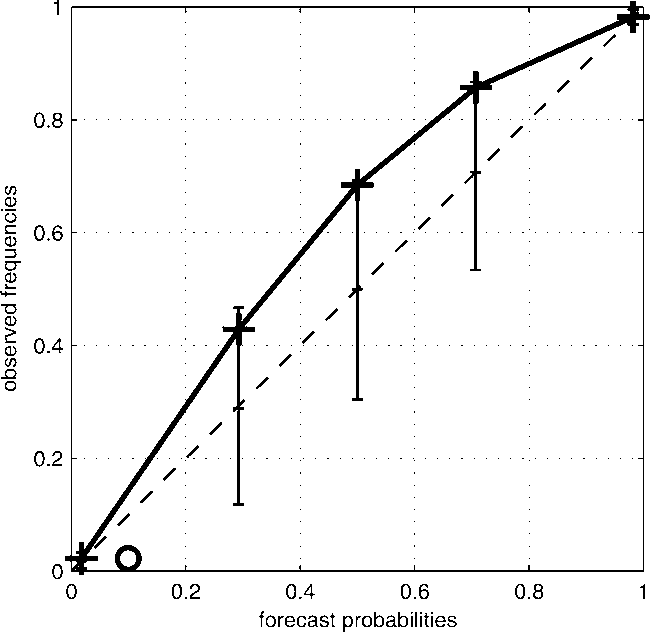
\includegraphics[width=0.45\textwidth]{figures/consistency_bars/reliability_diagram_with_bars_1.png}%
      \hspace{0.5cm}%
      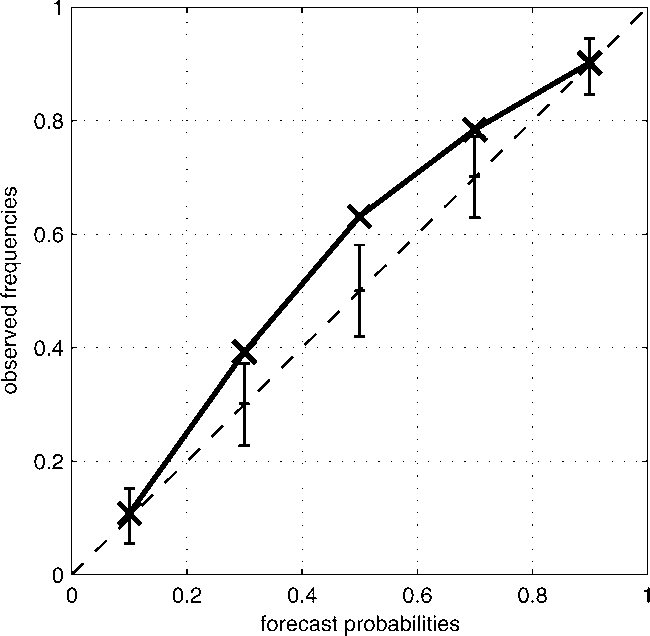
\includegraphics[width=0.45\textwidth]{figures/consistency_bars/reliability_diagram_with_bars_2.png}%
    }
  \end{tcolorbox}
  \reffootnote{Broecker2007}
\end{frame}

\begin{frame}{Variant}
  \begin{figure}
    \centering
    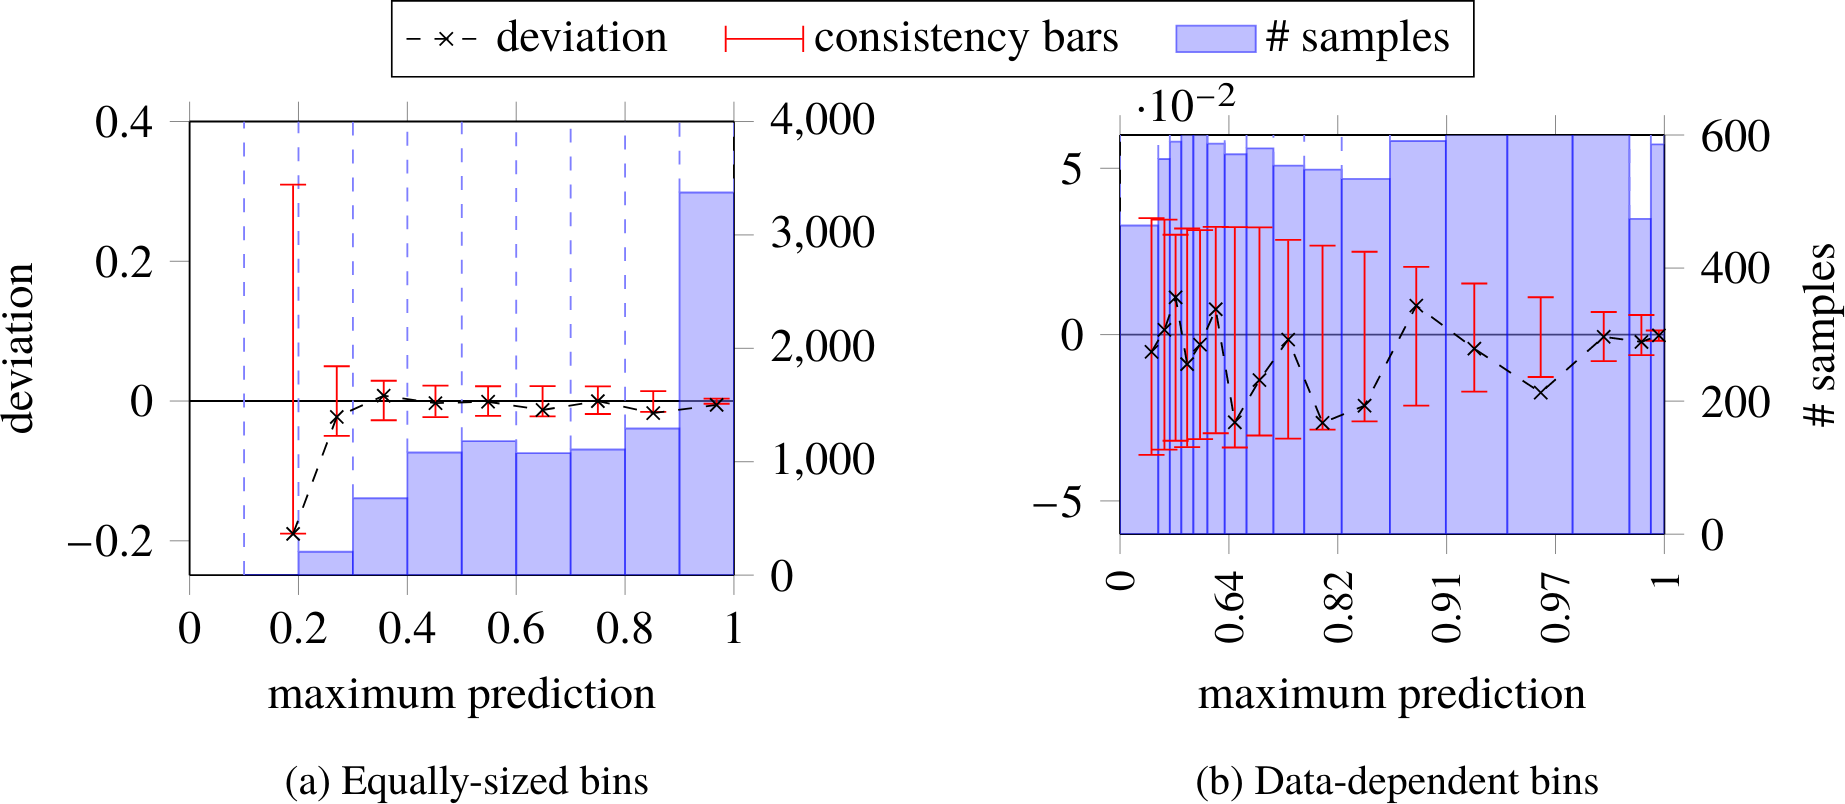
\includegraphics[width=0.9\textwidth]{figures/consistency_bars/variant.png}
  \end{figure}
  \reffootnote{Vaicenavicius2019}
\end{frame}

\begin{frame}{Kernel calibration error: Distribution-free tests}
  \begin{tcolorbox}[blankest,halign=flush center]
    \hl{Upper bound} the p-value
  \end{tcolorbox}
  \onslide<2->{%
    \tikzsetnextfilename{pvalues_distribution_free}
    \begin{tikzpicture}
\begin{groupplot}[group style={group size={3 by 3}, xlabels at={edge bottom}, ylabels at={edge left}, horizontal sep={0.1\linewidth}, vertical sep={0.023\linewidth}, xticklabels at={edge bottom}}, no markers, tick label style={font={\tiny}}, grid={major}, title style={align={center}}, width={0.3\linewidth}, height={0.17\linewidth}, every x tick scale label/.style={at={{(1,0)}}, anchor={west}}, ylabel style={font={\small}}, xmin={0}, xmax={1}, ymin={-0.1}, ymax={1.1}]
    \nextgroupplot[title={$\mathbf{M1}$}, ylabel={$\mathbf{D}_{\mathrm{b}}$}]
    \addplot+[thick]
        table[row sep={\\}]
        {
            \\
            0.0  0.0  \\
            0.01  0.0  \\
            0.02  0.0  \\
            0.03  0.0  \\
            0.04  0.0  \\
            0.05  0.0  \\
            0.06  0.0  \\
            0.07  0.0  \\
            0.08  0.0  \\
            0.09  0.0  \\
            0.1  0.0  \\
            0.11  0.0  \\
            0.12  0.0  \\
            0.13  0.0  \\
            0.14  0.0  \\
            0.15  0.0  \\
            0.16  0.0  \\
            0.17  0.0  \\
            0.18  0.0  \\
            0.19  0.0  \\
            0.2  0.0  \\
            0.21  0.0  \\
            0.22  0.0  \\
            0.23  0.0  \\
            0.24  0.0  \\
            0.25  0.0  \\
            0.26  0.0  \\
            0.27  0.0  \\
            0.28  0.0  \\
            0.29  0.0  \\
            0.3  0.0  \\
            0.31  0.0  \\
            0.32  0.0  \\
            0.33  0.0  \\
            0.34  0.0  \\
            0.35  0.0  \\
            0.36  0.0  \\
            0.37  0.0  \\
            0.38  0.0  \\
            0.39  0.0  \\
            0.4  0.0  \\
            0.41  0.0  \\
            0.42  0.0  \\
            0.43  0.0  \\
            0.44  0.0  \\
            0.45  0.0  \\
            0.46  0.0  \\
            0.47  0.0  \\
            0.48  0.0  \\
            0.49  0.0  \\
            0.5  0.0  \\
            0.51  0.0  \\
            0.52  0.0  \\
            0.53  0.0  \\
            0.54  0.0  \\
            0.55  0.0  \\
            0.56  0.0  \\
            0.57  0.0  \\
            0.58  0.0  \\
            0.59  0.0  \\
            0.6  0.0  \\
            0.61  0.0  \\
            0.62  0.0  \\
            0.63  0.0  \\
            0.64  0.0  \\
            0.65  0.0  \\
            0.66  0.0  \\
            0.67  0.0  \\
            0.68  0.0  \\
            0.69  0.0  \\
            0.7  0.0  \\
            0.71  0.0  \\
            0.72  0.0  \\
            0.73  0.0  \\
            0.74  0.0  \\
            0.75  0.0  \\
            0.76  0.0  \\
            0.77  0.0  \\
            0.78  0.0  \\
            0.79  0.0  \\
            0.8  0.0  \\
            0.81  0.0  \\
            0.82  0.0  \\
            0.83  0.0  \\
            0.84  0.0  \\
            0.85  0.0  \\
            0.86  0.0  \\
            0.87  0.0  \\
            0.88  0.0  \\
            0.89  0.0  \\
            0.9  0.0  \\
            0.91  0.0  \\
            0.92  0.0  \\
            0.93  0.0  \\
            0.94  0.0  \\
            0.95  0.0  \\
            0.96  0.0  \\
            0.97  0.0  \\
            0.98  0.0  \\
            0.99  0.0  \\
            1.0  1.0  \\
        }
        ;
    \addplot+[dashed, thick]
        coordinates {
            (0,0)
            (1,1)
        }
        ;
    \nextgroupplot[title={$\mathbf{M2}$}]
    \addplot+[thick]
        table[row sep={\\}]
        {
            \\
            0.0  1.0  \\
            0.01  0.9843  \\
            0.02  0.8808  \\
            0.03  0.6994  \\
            0.04  0.5196000000000001  \\
            0.05  0.37060000000000004  \\
            0.06  0.25970000000000004  \\
            0.07  0.18200000000000005  \\
            0.08  0.12390000000000001  \\
            0.09  0.08450000000000002  \\
            0.1  0.056599999999999984  \\
            0.11  0.03739999999999999  \\
            0.12  0.025900000000000034  \\
            0.13  0.015700000000000047  \\
            0.14  0.0121  \\
            0.15  0.008099999999999996  \\
            0.16  0.005199999999999982  \\
            0.17  0.0038000000000000256  \\
            0.18  0.0024999999999999467  \\
            0.19  0.0013999999999999568  \\
            0.2  0.0010000000000000009  \\
            0.21  0.0004999999999999449  \\
            0.22  0.00039999999999995595  \\
            0.23  9.999999999998899e-5  \\
            0.24  0.0  \\
            0.25  0.0  \\
            0.26  0.0  \\
            0.27  0.0  \\
            0.28  0.0  \\
            0.29  0.0  \\
            0.3  0.0  \\
            0.31  0.0  \\
            0.32  0.0  \\
            0.33  0.0  \\
            0.34  0.0  \\
            0.35  0.0  \\
            0.36  0.0  \\
            0.37  0.0  \\
            0.38  0.0  \\
            0.39  0.0  \\
            0.4  0.0  \\
            0.41  0.0  \\
            0.42  0.0  \\
            0.43  0.0  \\
            0.44  0.0  \\
            0.45  0.0  \\
            0.46  0.0  \\
            0.47  0.0  \\
            0.48  0.0  \\
            0.49  0.0  \\
            0.5  0.0  \\
            0.51  0.0  \\
            0.52  0.0  \\
            0.53  0.0  \\
            0.54  0.0  \\
            0.55  0.0  \\
            0.56  0.0  \\
            0.57  0.0  \\
            0.58  0.0  \\
            0.59  0.0  \\
            0.6  0.0  \\
            0.61  0.0  \\
            0.62  0.0  \\
            0.63  0.0  \\
            0.64  0.0  \\
            0.65  0.0  \\
            0.66  0.0  \\
            0.67  0.0  \\
            0.68  0.0  \\
            0.69  0.0  \\
            0.7  0.0  \\
            0.71  0.0  \\
            0.72  0.0  \\
            0.73  0.0  \\
            0.74  0.0  \\
            0.75  0.0  \\
            0.76  0.0  \\
            0.77  0.0  \\
            0.78  0.0  \\
            0.79  0.0  \\
            0.8  0.0  \\
            0.81  0.0  \\
            0.82  0.0  \\
            0.83  0.0  \\
            0.84  0.0  \\
            0.85  0.0  \\
            0.86  0.0  \\
            0.87  0.0  \\
            0.88  0.0  \\
            0.89  0.0  \\
            0.9  0.0  \\
            0.91  0.0  \\
            0.92  0.0  \\
            0.93  0.0  \\
            0.94  0.0  \\
            0.95  0.0  \\
            0.96  0.0  \\
            0.97  0.0  \\
            0.98  0.0  \\
            0.99  0.0  \\
            1.0  0.0  \\
        }
        ;
    \nextgroupplot[title={$\mathbf{M3}$}]
    \addplot+[thick]
        table[row sep={\\}]
        {
            \\
            0.0  1.0  \\
            0.01  1.0  \\
            0.02  1.0  \\
            0.03  1.0  \\
            0.04  1.0  \\
            0.05  1.0  \\
            0.06  1.0  \\
            0.07  1.0  \\
            0.08  1.0  \\
            0.09  1.0  \\
            0.1  1.0  \\
            0.11  1.0  \\
            0.12  1.0  \\
            0.13  1.0  \\
            0.14  1.0  \\
            0.15  1.0  \\
            0.16  1.0  \\
            0.17  1.0  \\
            0.18  1.0  \\
            0.19  1.0  \\
            0.2  1.0  \\
            0.21  1.0  \\
            0.22  1.0  \\
            0.23  1.0  \\
            0.24  1.0  \\
            0.25  1.0  \\
            0.26  1.0  \\
            0.27  1.0  \\
            0.28  1.0  \\
            0.29  1.0  \\
            0.3  1.0  \\
            0.31  1.0  \\
            0.32  1.0  \\
            0.33  1.0  \\
            0.34  1.0  \\
            0.35  1.0  \\
            0.36  1.0  \\
            0.37  1.0  \\
            0.38  1.0  \\
            0.39  1.0  \\
            0.4  1.0  \\
            0.41  1.0  \\
            0.42  1.0  \\
            0.43  1.0  \\
            0.44  1.0  \\
            0.45  1.0  \\
            0.46  1.0  \\
            0.47  1.0  \\
            0.48  1.0  \\
            0.49  1.0  \\
            0.5  1.0  \\
            0.51  1.0  \\
            0.52  1.0  \\
            0.53  1.0  \\
            0.54  1.0  \\
            0.55  1.0  \\
            0.56  1.0  \\
            0.57  1.0  \\
            0.58  1.0  \\
            0.59  1.0  \\
            0.6  1.0  \\
            0.61  1.0  \\
            0.62  1.0  \\
            0.63  1.0  \\
            0.64  1.0  \\
            0.65  1.0  \\
            0.66  1.0  \\
            0.67  1.0  \\
            0.68  0.9999  \\
            0.69  0.9998  \\
            0.7  0.9997  \\
            0.71  0.999  \\
            0.72  0.9977  \\
            0.73  0.9958  \\
            0.74  0.9918  \\
            0.75  0.9861  \\
            0.76  0.9772  \\
            0.77  0.9618  \\
            0.78  0.9407  \\
            0.79  0.903  \\
            0.8  0.8487  \\
            0.81  0.7797000000000001  \\
            0.82  0.6905  \\
            0.83  0.5806  \\
            0.84  0.4609  \\
            0.85  0.33730000000000004  \\
            0.86  0.2247  \\
            0.87  0.13119999999999998  \\
            0.88  0.0676  \\
            0.89  0.030200000000000005  \\
            0.9  0.011499999999999955  \\
            0.91  0.0034999999999999476  \\
            0.92  0.0008000000000000229  \\
            0.93  9.999999999998899e-5  \\
            0.94  0.0  \\
            0.95  0.0  \\
            0.96  0.0  \\
            0.97  0.0  \\
            0.98  0.0  \\
            0.99  0.0  \\
            1.0  0.0  \\
        }
        ;
    \nextgroupplot[ylabel={$\mathbf{D}_{\mathrm{uq}}$}]
    \addplot+[thick]
        table[row sep={\\}]
        {
            \\
            0.0  0.0  \\
            0.01  0.0  \\
            0.02  0.0  \\
            0.03  0.0  \\
            0.04  0.0  \\
            0.05  0.0  \\
            0.06  0.0  \\
            0.07  0.0  \\
            0.08  0.0  \\
            0.09  0.0  \\
            0.1  0.0  \\
            0.11  0.0  \\
            0.12  0.0  \\
            0.13  0.0  \\
            0.14  0.0  \\
            0.15  0.0  \\
            0.16  0.0  \\
            0.17  0.0  \\
            0.18  0.0  \\
            0.19  0.0  \\
            0.2  0.0  \\
            0.21  0.0  \\
            0.22  0.0  \\
            0.23  0.0  \\
            0.24  0.0  \\
            0.25  0.0  \\
            0.26  0.0  \\
            0.27  0.0  \\
            0.28  0.0  \\
            0.29  0.0  \\
            0.3  0.0  \\
            0.31  0.0  \\
            0.32  0.0  \\
            0.33  0.0  \\
            0.34  0.0  \\
            0.35  0.0  \\
            0.36  0.0  \\
            0.37  0.0  \\
            0.38  0.0  \\
            0.39  0.0  \\
            0.4  0.0  \\
            0.41  0.0  \\
            0.42  0.0  \\
            0.43  0.0  \\
            0.44  0.0  \\
            0.45  0.0  \\
            0.46  0.0  \\
            0.47  0.0  \\
            0.48  0.0  \\
            0.49  0.0  \\
            0.5  0.0  \\
            0.51  0.0  \\
            0.52  0.0  \\
            0.53  0.0  \\
            0.54  0.0  \\
            0.55  0.0  \\
            0.56  0.0  \\
            0.57  0.0  \\
            0.58  0.0  \\
            0.59  0.0  \\
            0.6  0.0  \\
            0.61  0.0  \\
            0.62  0.0  \\
            0.63  0.0  \\
            0.64  0.0  \\
            0.65  0.0  \\
            0.66  0.0  \\
            0.67  0.0  \\
            0.68  0.0  \\
            0.69  0.0  \\
            0.7  0.0  \\
            0.71  0.0  \\
            0.72  0.0  \\
            0.73  0.0  \\
            0.74  0.0  \\
            0.75  0.0  \\
            0.76  0.0  \\
            0.77  0.0  \\
            0.78  0.0  \\
            0.79  0.0  \\
            0.8  0.0  \\
            0.81  0.0  \\
            0.82  0.0  \\
            0.83  0.0  \\
            0.84  0.0  \\
            0.85  0.0  \\
            0.86  0.0  \\
            0.87  0.0  \\
            0.88  0.0  \\
            0.89  0.0  \\
            0.9  0.0  \\
            0.91  0.0  \\
            0.92  0.0  \\
            0.93  0.0  \\
            0.94  0.0  \\
            0.95  0.0  \\
            0.96  0.0  \\
            0.97  0.0  \\
            0.98  0.0  \\
            0.99  0.0  \\
            1.0  1.0  \\
        }
        ;
    \addplot+[dashed, thick]
        coordinates {
            (0,0)
            (1,1)
        }
        ;
    \nextgroupplot
    \addplot+[thick]
        table[row sep={\\}]
        {
            \\
            0.0  1.0  \\
            0.01  1.0  \\
            0.02  1.0  \\
            0.03  1.0  \\
            0.04  1.0  \\
            0.05  1.0  \\
            0.06  1.0  \\
            0.07  1.0  \\
            0.08  1.0  \\
            0.09  1.0  \\
            0.1  1.0  \\
            0.11  1.0  \\
            0.12  1.0  \\
            0.13  1.0  \\
            0.14  1.0  \\
            0.15  1.0  \\
            0.16  1.0  \\
            0.17  1.0  \\
            0.18  1.0  \\
            0.19  1.0  \\
            0.2  1.0  \\
            0.21  1.0  \\
            0.22  1.0  \\
            0.23  1.0  \\
            0.24  1.0  \\
            0.25  1.0  \\
            0.26  1.0  \\
            0.27  1.0  \\
            0.28  1.0  \\
            0.29  1.0  \\
            0.3  1.0  \\
            0.31  1.0  \\
            0.32  1.0  \\
            0.33  1.0  \\
            0.34  1.0  \\
            0.35  1.0  \\
            0.36  1.0  \\
            0.37  1.0  \\
            0.38  1.0  \\
            0.39  1.0  \\
            0.4  1.0  \\
            0.41  1.0  \\
            0.42  1.0  \\
            0.43  1.0  \\
            0.44  1.0  \\
            0.45  1.0  \\
            0.46  1.0  \\
            0.47  1.0  \\
            0.48  1.0  \\
            0.49  1.0  \\
            0.5  1.0  \\
            0.51  1.0  \\
            0.52  1.0  \\
            0.53  1.0  \\
            0.54  1.0  \\
            0.55  1.0  \\
            0.56  1.0  \\
            0.57  1.0  \\
            0.58  1.0  \\
            0.59  1.0  \\
            0.6  1.0  \\
            0.61  1.0  \\
            0.62  1.0  \\
            0.63  1.0  \\
            0.64  1.0  \\
            0.65  1.0  \\
            0.66  1.0  \\
            0.67  1.0  \\
            0.68  1.0  \\
            0.69  1.0  \\
            0.7  0.9999  \\
            0.71  0.9998  \\
            0.72  0.9997  \\
            0.73  0.9993  \\
            0.74  0.9982  \\
            0.75  0.9962  \\
            0.76  0.9931  \\
            0.77  0.9877  \\
            0.78  0.9818  \\
            0.79  0.9711  \\
            0.8  0.952  \\
            0.81  0.9261  \\
            0.82  0.8895  \\
            0.83  0.8322  \\
            0.84  0.7575000000000001  \\
            0.85  0.6692  \\
            0.86  0.5622  \\
            0.87  0.4465  \\
            0.88  0.32830000000000004  \\
            0.89  0.2278  \\
            0.9  0.13970000000000005  \\
            0.91  0.07399999999999995  \\
            0.92  0.03149999999999997  \\
            0.93  0.012199999999999989  \\
            0.94  0.0030999999999999917  \\
            0.95  0.00039999999999995595  \\
            0.96  0.0  \\
            0.97  0.0  \\
            0.98  0.0  \\
            0.99  0.0  \\
            1.0  0.0  \\
        }
        ;
    \nextgroupplot
    \addplot+[thick]
        table[row sep={\\}]
        {
            \\
            0.0  1.0  \\
            0.01  1.0  \\
            0.02  1.0  \\
            0.03  1.0  \\
            0.04  1.0  \\
            0.05  1.0  \\
            0.06  1.0  \\
            0.07  1.0  \\
            0.08  1.0  \\
            0.09  1.0  \\
            0.1  1.0  \\
            0.11  1.0  \\
            0.12  1.0  \\
            0.13  1.0  \\
            0.14  1.0  \\
            0.15  1.0  \\
            0.16  1.0  \\
            0.17  1.0  \\
            0.18  1.0  \\
            0.19  1.0  \\
            0.2  1.0  \\
            0.21  1.0  \\
            0.22  1.0  \\
            0.23  1.0  \\
            0.24  1.0  \\
            0.25  1.0  \\
            0.26  1.0  \\
            0.27  1.0  \\
            0.28  1.0  \\
            0.29  1.0  \\
            0.3  1.0  \\
            0.31  1.0  \\
            0.32  1.0  \\
            0.33  1.0  \\
            0.34  1.0  \\
            0.35  1.0  \\
            0.36  1.0  \\
            0.37  1.0  \\
            0.38  1.0  \\
            0.39  1.0  \\
            0.4  1.0  \\
            0.41  1.0  \\
            0.42  1.0  \\
            0.43  1.0  \\
            0.44  1.0  \\
            0.45  1.0  \\
            0.46  1.0  \\
            0.47  1.0  \\
            0.48  1.0  \\
            0.49  1.0  \\
            0.5  1.0  \\
            0.51  1.0  \\
            0.52  1.0  \\
            0.53  1.0  \\
            0.54  1.0  \\
            0.55  1.0  \\
            0.56  1.0  \\
            0.57  1.0  \\
            0.58  1.0  \\
            0.59  1.0  \\
            0.6  1.0  \\
            0.61  1.0  \\
            0.62  1.0  \\
            0.63  1.0  \\
            0.64  1.0  \\
            0.65  1.0  \\
            0.66  1.0  \\
            0.67  1.0  \\
            0.68  1.0  \\
            0.69  1.0  \\
            0.7  1.0  \\
            0.71  1.0  \\
            0.72  1.0  \\
            0.73  1.0  \\
            0.74  1.0  \\
            0.75  1.0  \\
            0.76  1.0  \\
            0.77  1.0  \\
            0.78  1.0  \\
            0.79  1.0  \\
            0.8  1.0  \\
            0.81  1.0  \\
            0.82  1.0  \\
            0.83  1.0  \\
            0.84  1.0  \\
            0.85  1.0  \\
            0.86  1.0  \\
            0.87  1.0  \\
            0.88  1.0  \\
            0.89  1.0  \\
            0.9  1.0  \\
            0.91  1.0  \\
            0.92  1.0  \\
            0.93  1.0  \\
            0.94  1.0  \\
            0.95  1.0  \\
            0.96  1.0  \\
            0.97  1.0  \\
            0.98  1.0  \\
            0.99  1.0  \\
            1.0  0.0  \\
        }
        ;
    \nextgroupplot[ylabel={$\mathbf{D}_{\mathrm{l}}$}]
    \addplot+[thick]
        table[row sep={\\}]
        {
            \\
            0.0  0.0  \\
            0.01  0.0  \\
            0.02  0.0  \\
            0.03  0.0  \\
            0.04  0.0  \\
            0.05  0.0  \\
            0.06  0.0  \\
            0.07  0.0  \\
            0.08  0.0  \\
            0.09  0.0  \\
            0.1  0.0  \\
            0.11  0.0  \\
            0.12  0.0  \\
            0.13  0.0  \\
            0.14  0.0  \\
            0.15  0.0  \\
            0.16  0.0  \\
            0.17  0.0  \\
            0.18  0.0  \\
            0.19  0.0  \\
            0.2  0.0  \\
            0.21  0.0  \\
            0.22  0.0  \\
            0.23  0.0  \\
            0.24  0.0  \\
            0.25  0.0  \\
            0.26  0.0  \\
            0.27  0.0  \\
            0.28  0.0  \\
            0.29  0.0  \\
            0.3  0.0  \\
            0.31  0.0  \\
            0.32  0.0  \\
            0.33  0.0  \\
            0.34  0.0  \\
            0.35  0.0  \\
            0.36  0.0  \\
            0.37  0.0  \\
            0.38  0.0  \\
            0.39  0.0  \\
            0.4  0.0  \\
            0.41  0.0  \\
            0.42  0.0  \\
            0.43  0.0  \\
            0.44  0.0  \\
            0.45  0.0  \\
            0.46  0.0  \\
            0.47  0.0  \\
            0.48  0.0  \\
            0.49  0.0  \\
            0.5  0.0  \\
            0.51  0.0  \\
            0.52  0.0  \\
            0.53  0.0  \\
            0.54  0.0  \\
            0.55  0.0  \\
            0.56  0.0  \\
            0.57  0.0  \\
            0.58  0.0  \\
            0.59  0.0  \\
            0.6  0.0  \\
            0.61  0.0  \\
            0.62  0.0  \\
            0.63  0.0  \\
            0.64  0.0  \\
            0.65  0.0  \\
            0.66  0.0  \\
            0.67  0.0  \\
            0.68  0.0  \\
            0.69  0.0  \\
            0.7  0.0  \\
            0.71  0.0  \\
            0.72  0.0  \\
            0.73  0.0  \\
            0.74  0.0  \\
            0.75  0.0  \\
            0.76  0.0  \\
            0.77  0.0  \\
            0.78  0.0  \\
            0.79  0.0  \\
            0.8  0.0  \\
            0.81  0.0  \\
            0.82  0.0  \\
            0.83  0.0  \\
            0.84  0.0  \\
            0.85  0.0  \\
            0.86  0.0  \\
            0.87  0.0  \\
            0.88  0.0  \\
            0.89  0.0  \\
            0.9  0.0  \\
            0.91  0.0  \\
            0.92  0.0  \\
            0.93  0.0  \\
            0.94  0.0  \\
            0.95  0.0  \\
            0.96  0.0  \\
            0.97  0.0  \\
            0.98  0.0  \\
            0.99  0.0006  \\
            1.0  1.0  \\
        }
        ;
    \addplot+[dashed, thick]
        coordinates {
            (0,0)
            (1,1)
        }
        ;
    \nextgroupplot
    \addplot+[thick]
        table[row sep={\\}]
        {
            \\
            0.0  1.0  \\
            0.01  1.0  \\
            0.02  1.0  \\
            0.03  1.0  \\
            0.04  1.0  \\
            0.05  1.0  \\
            0.06  1.0  \\
            0.07  1.0  \\
            0.08  1.0  \\
            0.09  1.0  \\
            0.1  1.0  \\
            0.11  1.0  \\
            0.12  1.0  \\
            0.13  1.0  \\
            0.14  1.0  \\
            0.15  1.0  \\
            0.16  1.0  \\
            0.17  1.0  \\
            0.18  1.0  \\
            0.19  1.0  \\
            0.2  1.0  \\
            0.21  1.0  \\
            0.22  1.0  \\
            0.23  1.0  \\
            0.24  1.0  \\
            0.25  1.0  \\
            0.26  1.0  \\
            0.27  1.0  \\
            0.28  1.0  \\
            0.29  1.0  \\
            0.3  1.0  \\
            0.31  1.0  \\
            0.32  1.0  \\
            0.33  1.0  \\
            0.34  1.0  \\
            0.35  1.0  \\
            0.36  1.0  \\
            0.37  1.0  \\
            0.38  1.0  \\
            0.39  1.0  \\
            0.4  1.0  \\
            0.41  1.0  \\
            0.42  1.0  \\
            0.43  1.0  \\
            0.44  1.0  \\
            0.45  1.0  \\
            0.46  1.0  \\
            0.47  1.0  \\
            0.48  1.0  \\
            0.49  1.0  \\
            0.5  1.0  \\
            0.51  1.0  \\
            0.52  1.0  \\
            0.53  1.0  \\
            0.54  1.0  \\
            0.55  1.0  \\
            0.56  1.0  \\
            0.57  1.0  \\
            0.58  1.0  \\
            0.59  1.0  \\
            0.6  1.0  \\
            0.61  0.9999  \\
            0.62  0.9997  \\
            0.63  0.9995  \\
            0.64  0.9993  \\
            0.65  0.9989  \\
            0.66  0.9987  \\
            0.67  0.9982  \\
            0.68  0.9973  \\
            0.69  0.9961  \\
            0.7  0.9951  \\
            0.71  0.9925  \\
            0.72  0.9888  \\
            0.73  0.985  \\
            0.74  0.9773  \\
            0.75  0.969  \\
            0.76  0.9596  \\
            0.77  0.9449  \\
            0.78  0.9262  \\
            0.79  0.9023  \\
            0.8  0.8748  \\
            0.81  0.836  \\
            0.82  0.7911  \\
            0.83  0.7404999999999999  \\
            0.84  0.6813  \\
            0.85  0.6166  \\
            0.86  0.5448  \\
            0.87  0.47019999999999995  \\
            0.88  0.39339999999999997  \\
            0.89  0.3164  \\
            0.9  0.23939999999999995  \\
            0.91  0.17420000000000002  \\
            0.92  0.11980000000000002  \\
            0.93  0.07279999999999998  \\
            0.94  0.03969999999999996  \\
            0.95  0.01870000000000005  \\
            0.96  0.007099999999999995  \\
            0.97  0.0022999999999999687  \\
            0.98  0.00039999999999995595  \\
            0.99  0.0  \\
            1.0  0.0  \\
        }
        ;
    \nextgroupplot
    \addplot+[thick]
        table[row sep={\\}]
        {
            \\
            0.0  1.0  \\
            0.01  1.0  \\
            0.02  1.0  \\
            0.03  1.0  \\
            0.04  1.0  \\
            0.05  1.0  \\
            0.06  1.0  \\
            0.07  1.0  \\
            0.08  1.0  \\
            0.09  1.0  \\
            0.1  1.0  \\
            0.11  1.0  \\
            0.12  1.0  \\
            0.13  1.0  \\
            0.14  1.0  \\
            0.15  1.0  \\
            0.16  1.0  \\
            0.17  1.0  \\
            0.18  1.0  \\
            0.19  1.0  \\
            0.2  1.0  \\
            0.21  1.0  \\
            0.22  1.0  \\
            0.23  1.0  \\
            0.24  1.0  \\
            0.25  1.0  \\
            0.26  1.0  \\
            0.27  1.0  \\
            0.28  1.0  \\
            0.29  1.0  \\
            0.3  1.0  \\
            0.31  1.0  \\
            0.32  1.0  \\
            0.33  1.0  \\
            0.34  1.0  \\
            0.35  1.0  \\
            0.36  1.0  \\
            0.37  1.0  \\
            0.38  1.0  \\
            0.39  1.0  \\
            0.4  1.0  \\
            0.41  1.0  \\
            0.42  1.0  \\
            0.43  1.0  \\
            0.44  1.0  \\
            0.45  1.0  \\
            0.46  1.0  \\
            0.47  1.0  \\
            0.48  1.0  \\
            0.49  1.0  \\
            0.5  1.0  \\
            0.51  1.0  \\
            0.52  1.0  \\
            0.53  1.0  \\
            0.54  1.0  \\
            0.55  1.0  \\
            0.56  1.0  \\
            0.57  1.0  \\
            0.58  1.0  \\
            0.59  1.0  \\
            0.6  1.0  \\
            0.61  1.0  \\
            0.62  1.0  \\
            0.63  1.0  \\
            0.64  1.0  \\
            0.65  1.0  \\
            0.66  1.0  \\
            0.67  1.0  \\
            0.68  1.0  \\
            0.69  1.0  \\
            0.7  1.0  \\
            0.71  1.0  \\
            0.72  1.0  \\
            0.73  1.0  \\
            0.74  1.0  \\
            0.75  1.0  \\
            0.76  1.0  \\
            0.77  1.0  \\
            0.78  1.0  \\
            0.79  1.0  \\
            0.8  1.0  \\
            0.81  1.0  \\
            0.82  1.0  \\
            0.83  1.0  \\
            0.84  1.0  \\
            0.85  1.0  \\
            0.86  0.9999  \\
            0.87  0.9999  \\
            0.88  0.9998  \\
            0.89  0.9998  \\
            0.9  0.9996  \\
            0.91  0.9993  \\
            0.92  0.9988  \\
            0.93  0.997  \\
            0.94  0.9937  \\
            0.95  0.9861  \\
            0.96  0.9711  \\
            0.97  0.9399  \\
            0.98  0.8691  \\
            0.99  0.7115  \\
            1.0  0.0  \\
        }
        ;
\end{groupplot}
\node[anchor=north] at ($(group c1r3.west |- group c1r3.outer south)!0.5!(group c3r3.east |- group c3r3.outer south)$){significance level};
\node[anchor=south, rotate=90] at ($(group c1r1.north -| group c1r1.outer west)!0.5!(group c1r3.south -| group c1r3.outer west)$){empirical test error};
\end{tikzpicture}%
  }
  \reffootnote{Widmann2019}
\end{frame}

\begin{frame}{Kernel calibration error: Asymptotic tests}
  \begin{tcolorbox}[blankest, halign=flush center]
    \hl{Approximate} the p-value based on the \hl{asymptotic} distribution
  \end{tcolorbox}
  \onslide<2->{%
    \tikzsetnextfilename{pvalues_asymptotic}
    \begin{tikzpicture}
\begin{groupplot}[group style={group size={3 by 2}, xlabels at={edge bottom}, ylabels at={edge left}, horizontal sep={0.1\linewidth}, vertical sep={0.023\linewidth}, xticklabels at={edge bottom}}, no markers, tick label style={font={\tiny}}, grid={major}, title style={align={center}}, width={0.3\linewidth}, height={0.17\linewidth}, every x tick scale label/.style={at={{(1,0)}}, anchor={west}}, ylabel style={font={\small}}, xmin={0}, xmax={1}, ymin={-0.1}, ymax={1.1}]
    \nextgroupplot[title={$\mathbf{M1}$}, ylabel={$\mathbf{A}_{\mathrm{uq}}$}]
    \addplot+[thick]
        table[row sep={\\}]
        {
            \\
            0.0  0.0002  \\
            0.01  0.0048  \\
            0.02  0.0123  \\
            0.03  0.0194  \\
            0.04  0.0257  \\
            0.05  0.0347  \\
            0.06  0.0452  \\
            0.07  0.0536  \\
            0.08  0.0616  \\
            0.09  0.0708  \\
            0.1  0.0791  \\
            0.11  0.0907  \\
            0.12  0.1002  \\
            0.13  0.1102  \\
            0.14  0.1196  \\
            0.15  0.1296  \\
            0.16  0.1391  \\
            0.17  0.148  \\
            0.18  0.1597  \\
            0.19  0.1697  \\
            0.2  0.181  \\
            0.21  0.1927  \\
            0.22  0.2021  \\
            0.23  0.2127  \\
            0.24  0.2247  \\
            0.25  0.2364  \\
            0.26  0.2485  \\
            0.27  0.258  \\
            0.28  0.2691  \\
            0.29  0.2782  \\
            0.3  0.2893  \\
            0.31  0.301  \\
            0.32  0.3138  \\
            0.33  0.324  \\
            0.34  0.3354  \\
            0.35  0.3458  \\
            0.36  0.3576  \\
            0.37  0.3666  \\
            0.38  0.3784  \\
            0.39  0.3899  \\
            0.4  0.4019  \\
            0.41  0.4139  \\
            0.42  0.425  \\
            0.43  0.4357  \\
            0.44  0.445  \\
            0.45  0.4567  \\
            0.46  0.468  \\
            0.47  0.4778  \\
            0.48  0.4869  \\
            0.49  0.5007  \\
            0.5  0.5111  \\
            0.51  0.5238  \\
            0.52  0.5348  \\
            0.53  0.545  \\
            0.54  0.5543  \\
            0.55  0.5645  \\
            0.56  0.5747  \\
            0.57  0.5872  \\
            0.58  0.598  \\
            0.59  0.6095  \\
            0.6  0.6209  \\
            0.61  0.6323  \\
            0.62  0.6416  \\
            0.63  0.6518  \\
            0.64  0.6624  \\
            0.65  0.6747  \\
            0.66  0.6849  \\
            0.67  0.6949  \\
            0.68  0.7052  \\
            0.69  0.7159  \\
            0.7  0.7271  \\
            0.71  0.7382  \\
            0.72  0.7475  \\
            0.73  0.7594  \\
            0.74  0.7708  \\
            0.75  0.7826  \\
            0.76  0.7928  \\
            0.77  0.805  \\
            0.78  0.816  \\
            0.79  0.8256  \\
            0.8  0.8366  \\
            0.81  0.8472  \\
            0.82  0.8585  \\
            0.83  0.8688  \\
            0.84  0.8799  \\
            0.85  0.8888  \\
            0.86  0.8987  \\
            0.87  0.9097  \\
            0.88  0.9188  \\
            0.89  0.9269  \\
            0.9  0.9366  \\
            0.91  0.9448  \\
            0.92  0.9535  \\
            0.93  0.9612  \\
            0.94  0.9687  \\
            0.95  0.9761  \\
            0.96  0.9815  \\
            0.97  0.9884  \\
            0.98  0.9942  \\
            0.99  0.998  \\
            1.0  1.0  \\
        }
        ;
    \addplot+[dashed, thick]
        coordinates {
            (0,0)
            (1,1)
        }
        ;
    \nextgroupplot[title={$\mathbf{M2}$}]
    \addplot+[thick]
        table[row sep={\\}]
        {
            \\
            0.0  0.0  \\
            0.01  0.0  \\
            0.02  0.0  \\
            0.03  0.0  \\
            0.04  0.0  \\
            0.05  0.0  \\
            0.06  0.0  \\
            0.07  0.0  \\
            0.08  0.0  \\
            0.09  0.0  \\
            0.1  0.0  \\
            0.11  0.0  \\
            0.12  0.0  \\
            0.13  0.0  \\
            0.14  0.0  \\
            0.15  0.0  \\
            0.16  0.0  \\
            0.17  0.0  \\
            0.18  0.0  \\
            0.19  0.0  \\
            0.2  0.0  \\
            0.21  0.0  \\
            0.22  0.0  \\
            0.23  0.0  \\
            0.24  0.0  \\
            0.25  0.0  \\
            0.26  0.0  \\
            0.27  0.0  \\
            0.28  0.0  \\
            0.29  0.0  \\
            0.3  0.0  \\
            0.31  0.0  \\
            0.32  0.0  \\
            0.33  0.0  \\
            0.34  0.0  \\
            0.35  0.0  \\
            0.36  0.0  \\
            0.37  0.0  \\
            0.38  0.0  \\
            0.39  0.0  \\
            0.4  0.0  \\
            0.41  0.0  \\
            0.42  0.0  \\
            0.43  0.0  \\
            0.44  0.0  \\
            0.45  0.0  \\
            0.46  0.0  \\
            0.47  0.0  \\
            0.48  0.0  \\
            0.49  0.0  \\
            0.5  0.0  \\
            0.51  0.0  \\
            0.52  0.0  \\
            0.53  0.0  \\
            0.54  0.0  \\
            0.55  0.0  \\
            0.56  0.0  \\
            0.57  0.0  \\
            0.58  0.0  \\
            0.59  0.0  \\
            0.6  0.0  \\
            0.61  0.0  \\
            0.62  0.0  \\
            0.63  0.0  \\
            0.64  0.0  \\
            0.65  0.0  \\
            0.66  0.0  \\
            0.67  0.0  \\
            0.68  0.0  \\
            0.69  0.0  \\
            0.7  0.0  \\
            0.71  0.0  \\
            0.72  0.0  \\
            0.73  0.0  \\
            0.74  0.0  \\
            0.75  0.0  \\
            0.76  0.0  \\
            0.77  0.0  \\
            0.78  0.0  \\
            0.79  0.0  \\
            0.8  0.0  \\
            0.81  0.0  \\
            0.82  0.0  \\
            0.83  0.0  \\
            0.84  0.0  \\
            0.85  0.0  \\
            0.86  0.0  \\
            0.87  0.0  \\
            0.88  0.0  \\
            0.89  0.0  \\
            0.9  0.0  \\
            0.91  0.0  \\
            0.92  0.0  \\
            0.93  0.0  \\
            0.94  0.0  \\
            0.95  0.0  \\
            0.96  0.0  \\
            0.97  0.0  \\
            0.98  0.0  \\
            0.99  0.0  \\
            1.0  0.0  \\
        }
        ;
    \nextgroupplot[title={$\mathbf{M3}$}]
    \addplot+[thick]
        table[row sep={\\}]
        {
            \\
            0.0  0.0  \\
            0.01  0.0  \\
            0.02  0.0  \\
            0.03  0.0  \\
            0.04  0.0  \\
            0.05  0.0  \\
            0.06  0.0  \\
            0.07  0.0  \\
            0.08  0.0  \\
            0.09  0.0  \\
            0.1  0.0  \\
            0.11  0.0  \\
            0.12  0.0  \\
            0.13  0.0  \\
            0.14  0.0  \\
            0.15  0.0  \\
            0.16  0.0  \\
            0.17  0.0  \\
            0.18  0.0  \\
            0.19  0.0  \\
            0.2  0.0  \\
            0.21  0.0  \\
            0.22  0.0  \\
            0.23  0.0  \\
            0.24  0.0  \\
            0.25  0.0  \\
            0.26  0.0  \\
            0.27  0.0  \\
            0.28  0.0  \\
            0.29  0.0  \\
            0.3  0.0  \\
            0.31  0.0  \\
            0.32  0.0  \\
            0.33  0.0  \\
            0.34  0.0  \\
            0.35  0.0  \\
            0.36  0.0  \\
            0.37  0.0  \\
            0.38  0.0  \\
            0.39  0.0  \\
            0.4  0.0  \\
            0.41  0.0  \\
            0.42  0.0  \\
            0.43  0.0  \\
            0.44  0.0  \\
            0.45  0.0  \\
            0.46  0.0  \\
            0.47  0.0  \\
            0.48  0.0  \\
            0.49  0.0  \\
            0.5  0.0  \\
            0.51  0.0  \\
            0.52  0.0  \\
            0.53  0.0  \\
            0.54  0.0  \\
            0.55  0.0  \\
            0.56  0.0  \\
            0.57  0.0  \\
            0.58  0.0  \\
            0.59  0.0  \\
            0.6  0.0  \\
            0.61  0.0  \\
            0.62  0.0  \\
            0.63  0.0  \\
            0.64  0.0  \\
            0.65  0.0  \\
            0.66  0.0  \\
            0.67  0.0  \\
            0.68  0.0  \\
            0.69  0.0  \\
            0.7  0.0  \\
            0.71  0.0  \\
            0.72  0.0  \\
            0.73  0.0  \\
            0.74  0.0  \\
            0.75  0.0  \\
            0.76  0.0  \\
            0.77  0.0  \\
            0.78  0.0  \\
            0.79  0.0  \\
            0.8  0.0  \\
            0.81  0.0  \\
            0.82  0.0  \\
            0.83  0.0  \\
            0.84  0.0  \\
            0.85  0.0  \\
            0.86  0.0  \\
            0.87  0.0  \\
            0.88  0.0  \\
            0.89  0.0  \\
            0.9  0.0  \\
            0.91  0.0  \\
            0.92  0.0  \\
            0.93  0.0  \\
            0.94  0.0  \\
            0.95  0.0  \\
            0.96  0.0  \\
            0.97  0.0  \\
            0.98  0.0  \\
            0.99  0.0  \\
            1.0  0.0  \\
        }
        ;
    \nextgroupplot[ylabel={$\mathbf{A}_{\mathrm{l}}$}]
    \addplot+[thick]
        table[row sep={\\}]
        {
            \\
            0.0  0.0  \\
            0.01  0.0077  \\
            0.02  0.0162  \\
            0.03  0.0252  \\
            0.04  0.0353  \\
            0.05  0.0455  \\
            0.06  0.056  \\
            0.07  0.0656  \\
            0.08  0.0773  \\
            0.09  0.0868  \\
            0.1  0.098  \\
            0.11  0.1097  \\
            0.12  0.1186  \\
            0.13  0.1275  \\
            0.14  0.1394  \\
            0.15  0.1491  \\
            0.16  0.1598  \\
            0.17  0.1695  \\
            0.18  0.1798  \\
            0.19  0.191  \\
            0.2  0.2014  \\
            0.21  0.2126  \\
            0.22  0.2227  \\
            0.23  0.2327  \\
            0.24  0.243  \\
            0.25  0.2564  \\
            0.26  0.267  \\
            0.27  0.2759  \\
            0.28  0.2862  \\
            0.29  0.2973  \\
            0.3  0.3076  \\
            0.31  0.3182  \\
            0.32  0.3307  \\
            0.33  0.3402  \\
            0.34  0.3508  \\
            0.35  0.3607  \\
            0.36  0.3718  \\
            0.37  0.3801  \\
            0.38  0.3921  \\
            0.39  0.4033  \\
            0.4  0.4141  \\
            0.41  0.4244  \\
            0.42  0.4334  \\
            0.43  0.4441  \\
            0.44  0.4545  \\
            0.45  0.4647  \\
            0.46  0.4737  \\
            0.47  0.4836  \\
            0.48  0.4943  \\
            0.49  0.5037  \\
            0.5  0.5154  \\
            0.51  0.5236  \\
            0.52  0.5318  \\
            0.53  0.541  \\
            0.54  0.5513  \\
            0.55  0.5606  \\
            0.56  0.5707  \\
            0.57  0.5802  \\
            0.58  0.5899  \\
            0.59  0.5983  \\
            0.6  0.6075  \\
            0.61  0.616  \\
            0.62  0.625  \\
            0.63  0.6337  \\
            0.64  0.6431  \\
            0.65  0.6511  \\
            0.66  0.6614  \\
            0.67  0.6705  \\
            0.68  0.6794  \\
            0.69  0.6871  \\
            0.7  0.6957  \\
            0.71  0.7055  \\
            0.72  0.7152  \\
            0.73  0.7262  \\
            0.74  0.7358  \\
            0.75  0.7433  \\
            0.76  0.7521  \\
            0.77  0.7631  \\
            0.78  0.7724  \\
            0.79  0.781  \\
            0.8  0.7894  \\
            0.81  0.8002  \\
            0.82  0.81  \\
            0.83  0.8193  \\
            0.84  0.8282  \\
            0.85  0.8371  \\
            0.86  0.8452  \\
            0.87  0.8565  \\
            0.88  0.8678  \\
            0.89  0.8781  \\
            0.9  0.8906  \\
            0.91  0.9011  \\
            0.92  0.9121  \\
            0.93  0.9224  \\
            0.94  0.9324  \\
            0.95  0.9425  \\
            0.96  0.9523  \\
            0.97  0.9655  \\
            0.98  0.9774  \\
            0.99  0.9887  \\
            1.0  1.0  \\
        }
        ;
    \addplot+[dashed, thick]
        coordinates {
            (0,0)
            (1,1)
        }
        ;
    \nextgroupplot
    \addplot+[thick]
        table[row sep={\\}]
        {
            \\
            0.0  1.0  \\
            0.01  0.00039999999999995595  \\
            0.02  9.999999999998899e-5  \\
            0.03  0.0  \\
            0.04  0.0  \\
            0.05  0.0  \\
            0.06  0.0  \\
            0.07  0.0  \\
            0.08  0.0  \\
            0.09  0.0  \\
            0.1  0.0  \\
            0.11  0.0  \\
            0.12  0.0  \\
            0.13  0.0  \\
            0.14  0.0  \\
            0.15  0.0  \\
            0.16  0.0  \\
            0.17  0.0  \\
            0.18  0.0  \\
            0.19  0.0  \\
            0.2  0.0  \\
            0.21  0.0  \\
            0.22  0.0  \\
            0.23  0.0  \\
            0.24  0.0  \\
            0.25  0.0  \\
            0.26  0.0  \\
            0.27  0.0  \\
            0.28  0.0  \\
            0.29  0.0  \\
            0.3  0.0  \\
            0.31  0.0  \\
            0.32  0.0  \\
            0.33  0.0  \\
            0.34  0.0  \\
            0.35  0.0  \\
            0.36  0.0  \\
            0.37  0.0  \\
            0.38  0.0  \\
            0.39  0.0  \\
            0.4  0.0  \\
            0.41  0.0  \\
            0.42  0.0  \\
            0.43  0.0  \\
            0.44  0.0  \\
            0.45  0.0  \\
            0.46  0.0  \\
            0.47  0.0  \\
            0.48  0.0  \\
            0.49  0.0  \\
            0.5  0.0  \\
            0.51  0.0  \\
            0.52  0.0  \\
            0.53  0.0  \\
            0.54  0.0  \\
            0.55  0.0  \\
            0.56  0.0  \\
            0.57  0.0  \\
            0.58  0.0  \\
            0.59  0.0  \\
            0.6  0.0  \\
            0.61  0.0  \\
            0.62  0.0  \\
            0.63  0.0  \\
            0.64  0.0  \\
            0.65  0.0  \\
            0.66  0.0  \\
            0.67  0.0  \\
            0.68  0.0  \\
            0.69  0.0  \\
            0.7  0.0  \\
            0.71  0.0  \\
            0.72  0.0  \\
            0.73  0.0  \\
            0.74  0.0  \\
            0.75  0.0  \\
            0.76  0.0  \\
            0.77  0.0  \\
            0.78  0.0  \\
            0.79  0.0  \\
            0.8  0.0  \\
            0.81  0.0  \\
            0.82  0.0  \\
            0.83  0.0  \\
            0.84  0.0  \\
            0.85  0.0  \\
            0.86  0.0  \\
            0.87  0.0  \\
            0.88  0.0  \\
            0.89  0.0  \\
            0.9  0.0  \\
            0.91  0.0  \\
            0.92  0.0  \\
            0.93  0.0  \\
            0.94  0.0  \\
            0.95  0.0  \\
            0.96  0.0  \\
            0.97  0.0  \\
            0.98  0.0  \\
            0.99  0.0  \\
            1.0  0.0  \\
        }
        ;
    \nextgroupplot
    \addplot+[thick]
        table[row sep={\\}]
        {
            \\
            0.0  1.0  \\
            0.01  0.9519  \\
            0.02  0.911  \\
            0.03  0.8747  \\
            0.04  0.8446  \\
            0.05  0.8141  \\
            0.06  0.786  \\
            0.07  0.7593  \\
            0.08  0.7351  \\
            0.09  0.712  \\
            0.1  0.6896  \\
            0.11  0.6687000000000001  \\
            0.12  0.6483  \\
            0.13  0.6287  \\
            0.14  0.609  \\
            0.15  0.5924  \\
            0.16  0.5738  \\
            0.17  0.5589  \\
            0.18  0.5437000000000001  \\
            0.19  0.5274  \\
            0.2  0.5111  \\
            0.21  0.4961  \\
            0.22  0.4789  \\
            0.23  0.4648  \\
            0.24  0.4524  \\
            0.25  0.4395  \\
            0.26  0.4262  \\
            0.27  0.41459999999999997  \\
            0.28  0.40080000000000005  \\
            0.29  0.389  \\
            0.3  0.3771  \\
            0.31  0.3669  \\
            0.32  0.356  \\
            0.33  0.3477  \\
            0.34  0.3379  \\
            0.35  0.32789999999999997  \\
            0.36  0.3184  \\
            0.37  0.30800000000000005  \\
            0.38  0.2984  \\
            0.39  0.2884  \\
            0.4  0.2811  \\
            0.41  0.27370000000000005  \\
            0.42  0.26570000000000005  \\
            0.43  0.2571  \\
            0.44  0.24980000000000002  \\
            0.45  0.24229999999999996  \\
            0.46  0.2349  \\
            0.47  0.2267  \\
            0.48  0.21930000000000005  \\
            0.49  0.2128  \\
            0.5  0.20540000000000003  \\
            0.51  0.20030000000000003  \\
            0.52  0.19379999999999997  \\
            0.53  0.18799999999999994  \\
            0.54  0.1825  \\
            0.55  0.17459999999999998  \\
            0.56  0.16810000000000003  \\
            0.57  0.16190000000000004  \\
            0.58  0.1562  \\
            0.59  0.1511  \\
            0.6  0.14590000000000003  \\
            0.61  0.14039999999999997  \\
            0.62  0.13439999999999996  \\
            0.63  0.13029999999999997  \\
            0.64  0.12539999999999996  \\
            0.65  0.121  \\
            0.66  0.11670000000000003  \\
            0.67  0.11170000000000002  \\
            0.68  0.10699999999999998  \\
            0.69  0.10150000000000003  \\
            0.7  0.09740000000000004  \\
            0.71  0.09260000000000002  \\
            0.72  0.08840000000000003  \\
            0.73  0.08420000000000005  \\
            0.74  0.07950000000000002  \\
            0.75  0.07589999999999997  \\
            0.76  0.07169999999999999  \\
            0.77  0.06689999999999996  \\
            0.78  0.06359999999999999  \\
            0.79  0.06000000000000005  \\
            0.8  0.056599999999999984  \\
            0.81  0.0534  \\
            0.82  0.05020000000000002  \\
            0.83  0.04600000000000004  \\
            0.84  0.041200000000000014  \\
            0.85  0.03839999999999999  \\
            0.86  0.03539999999999999  \\
            0.87  0.03259999999999996  \\
            0.88  0.02969999999999995  \\
            0.89  0.0262  \\
            0.9  0.022599999999999953  \\
            0.91  0.020100000000000007  \\
            0.92  0.017299999999999982  \\
            0.93  0.014900000000000024  \\
            0.94  0.012800000000000034  \\
            0.95  0.009800000000000031  \\
            0.96  0.007600000000000051  \\
            0.97  0.005600000000000049  \\
            0.98  0.0038000000000000256  \\
            0.99  0.0020999999999999908  \\
            1.0  0.0  \\
        }
        ;
\end{groupplot}
\node[anchor=north] at ($(group c1r2.west |- group c1r2.outer south)!0.5!(group c3r2.east |- group c3r2.outer south)$){significance level};
\node[anchor=south, rotate=90] at ($(group c1r1.north -| group c1r1.outer west)!0.5!(group c1r2.south -| group c1r2.outer west)$){empirical test error};
\end{tikzpicture}%
  }
  \reffootnote{Widmann2019}
\end{frame}

\section{Calibration: Software packages}
\frame{\sectionpage}

\begin{frame}[fragile]{\texttt{CalibrationAnalysis.jl}}
  \begin{block}{Summary}
    \begin{itemize}
      \item Suite for analyzing calibration of probabilistic predictive models
      \item Written in Julia, with interfaces in Python (\texttt{pycalibration}) and R (\texttt{rcalibration})
    \end{itemize}
  \end{block}
  \pause
  \begin{block}{Features}
    \begin{itemize}
      \item Supports classification and regression models
      \item Reliability diagrams (\texttt{ReliabilityDiagrams.jl})
      \item Estimation of calibration errors such as ECE and KCE (\texttt{CalibrationErrors.jl})
      \item Calibration tests (\texttt{CalibrationTests.jl})
      \item Integration with Julia ecosystem: Supports \texttt{Plots.jl} and \texttt{Makie.jl}, \texttt{KernelFunctions.jl}, and \texttt{HypothesisTests.jl}
    \end{itemize}
  \end{block}
\end{frame}

\begin{frame}{Calibration analysis: Penguins example}
  We train a naive Bayes classifier of penguin species based on bill depth, bill length, flipper length, and body mass.
  \begin{figure}
    \centering
    \includegraphics[width=\textwidth]{figures/penguins/penguins.pdf}
  \end{figure}
\end{frame}

\begin{frame}{Binary predictions}
  \begin{figure}
    \centering
    \includegraphics[width=\textwidth]{figures/penguins/confidence.pdf}
  \end{figure}
\end{frame}

\begin{frame}[fragile]{Reliability diagram}
  \begin{columns}[t]
    \begin{column}{0.5\textwidth}
      \begin{block}{Code}
        \begin{juliaconsnippet}
julia> using CalibrationAnalysis, CairoMakie

julia> reliability(
           confidence,
           outcome;
           binning=EqualMass(; n=15),
           deviation=true,
           consistencybars=ConsistencyBars(),
      )
        \end{juliaconsnippet}
      \end{block}
    \end{column}
    \begin{column}{0.5\textwidth}
      \begin{block}{Polished result}
        \begin{figure}
          \centering
          \includegraphics[width=\textwidth]{figures/penguins/reliability_diagram.pdf}
        \end{figure}
      \end{block}
    \end{column}
  \end{columns}
\end{frame}

\begin{frame}[fragile]{Expected calibration error: Code}
  \begin{juliaconsnippet}
julia> ece = ECE(UniformBinning(5), TotalVariation());

julia> ece(confidence, outcome)
0.06594437403598197

julia> ece(predictions, observations)
0.15789651955832515
  \end{juliaconsnippet}
\end{frame}


\begin{frame}[fragile]{Kernel calibration error: Code}
  \begin{juliaconsnippet}
julia> kernel = GaussianKernel() ⊗ WhiteKernel();

julia> skce = SKCE(kernel);

julia> skce(predictions, observations)
0.0032631144705774404

julia> skce = SKCE(kernel; unbiased=false);

julia> skce(predictions, observations)
0.004202113116841622

julia> skce = SKCE(kernel; blocksize=5);

julia> skce(predictions, observations)
-0.005037270862051889
  \end{juliaconsnippet}
\end{frame}

\begin{frame}[fragile]{Calibration test: Code}
  \begin{juliaconsnippet}
julia> AsymptoticSKCETest(kernel, predictions, observations)
Asymptotic SKCE test
--------------------
Population details:
    parameter of interest:   SKCE
    value under h_0:         0.0
    point estimate:          0.00326311

Test summary:
    outcome with 95% confidence: reject h_0
    one-sided p-value:           0.0150

Details:
    test statistic: -0.0009060378940361157

julia> test = ConsistencyTest(ece, predictions, observations);

julia> pvalue(test; bootstrap_iters=10_000)
0.0188
  \end{juliaconsnippet}
\end{frame}

\begin{frame}{Additional resources}
  \begin{itemize}
    \item Online documentation: \url{https://devmotion.github.io/CalibrationErrors.jl/}
    \item Talk at JuliaCon 2021: \url{https://youtu.be/PrLsXFvwzuA}
          \begin{figure}
            \centering
            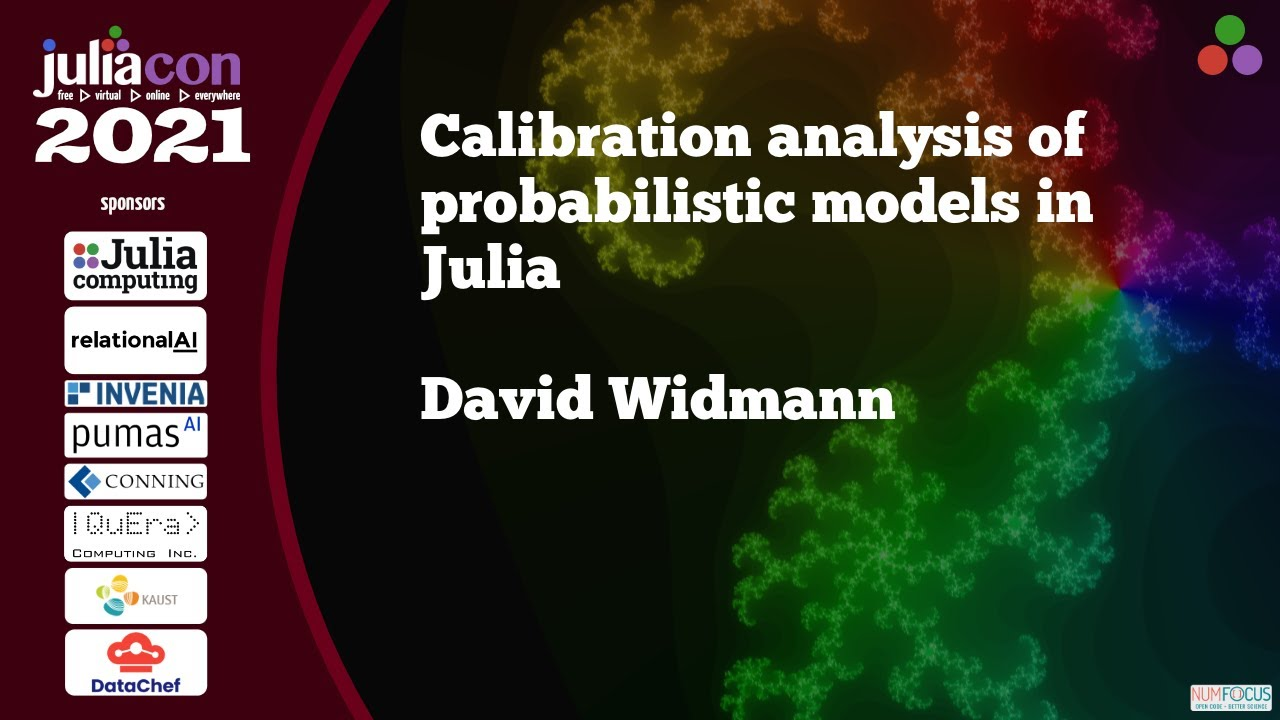
\includegraphics[height=0.5\textheight]{figures/youtube.jpg}
          \end{figure}
          Slides available at \url{https://talks.widmann.dev/2021/07/calibration/}
  \end{itemize}
\end{frame}

\section{Concluding remarks}
\frame{\sectionpage}

\begin{frame}{Important takeaways}
  \begin{itemize}
    \item More fine-grained analysis of calibration can be important
    \item MMD-like kernel calibration error can be applied to probabilistic models beyond classification
    \item Estimators of kernel calibration error have appealing properties
    \item Calibration errors and reliability diagrams can be misleading
  \end{itemize}
\end{frame}

\end{document}
